
%برای گزارشات ماهانه mscR و برای نسخه نهایی msc انتخاب شود
\documentclass[oneside,openany,bsc]{AUT-Thesis}
% در این فایل، دستورها و تنظیمات مورد نیاز، آورده شده است.
%-------------------------------------------------------------------------------------------------------------------
\usepackage {indentfirst}
\usepackage{multirow}
% در ورژن جدید زی‌پرشین برای تایپ متن‌های ریاضی، این سه بسته، حتماً باید فراخوانی شود
\usepackage{amsthm,amssymb,amsmath}

\usepackage{xcolor,colortbl}
\definecolor{Gray}{gray}{0.85}

% فراخوانی بسته زی‌پرشین و تعریف قلم فارسی و انگلیسی

% بسته‌ای برای تنطیم حاشیه‌های بالا، پایین، چپ و راست صفحه
\usepackage[top=35mm, bottom=37mm, left=25mm, right=30mm]{geometry}
% بسته‌‌ای برای ظاهر شدن شکل‌ها و تصاویر متن
\usepackage{graphicx}
% بسته‌ای برای رسم کادر
\usepackage{framed} 

% بسته‌‌ای برای چاپ شدن خودکار تعداد صفحات در صفحه «معرفی پایان‌نامه»

\usepackage{lastpage}
% بسته‌ و دستوراتی برای ایجاد لینک‌های رنگی با امکان جهش
%\usepackage[pagebackref=false,colorlinks,linkcolor=blue,citecolor=blue]{hyperref}
% چنانچه قصد پرینت گرفتن نوشته خود را دارید، خط بالا را غیرفعال و  از دستور زیر استفاده کنید چون در صورت استفاده از دستور زیر‌‌، 
% لینک‌ها به رنگ سیاه ظاهر خواهند شد که برای پرینت گرفتن، مناسب‌تر است
\usepackage[pagebackref=false]{hyperref}
% بسته‌ لازم برای تنظیم سربرگ‌ها
\usepackage{fancyhdr}
%
\usepackage[toc,page]{appendix} %appendix
\usepackage{setspace}
\usepackage{algorithm}
\usepackage{algorithmic}

\usepackage{subfigure}
\usepackage[subfigure,titles]{tocloft}
\cftsetindents{figure}{0em}{3.5em}
\cftsetindents{table}{0em}{3.5em}

% CONFLICT with SUBFIGURE !
%\usepackage{subcaption}
   %\captionsetup{textfont = sl} % use slanted font shape automatically for all captions
%\usepackage[noabbrev]{cleveref}

\usepackage{caption}
\captionsetup[table]{labelsep=space}
\captionsetup[figure]{labelsep=space}
\captionsetup[table]{position=top}   %% or below




% بسته‌ای برای ظاهر شدن «مراجع» و «نمایه» در فهرست مطالب
\usepackage[nottoc,notlof,notlot]{tocbibind}


% دستورات مربوط به ایجاد نمایه
\usepackage{makeidx}
\makeindex
%%%%%%%%%%%%%%%%%%%%%%%%%%
\usepackage{backnaur}

\usepackage{longtable}
\usepackage{titlesec}
\usepackage {graphicx}
\usepackage[Kashida=on, extrafootnotefeatures]{xepersian}

\settextfont[Scale=1]{XB Niloofar}
%\settextfont[Scale=0.9]{Persian Modern}
%\settextfont[Scale=1]{HM FElmi}
\setlatintextfont[Scale=0.9]{Latin Modern Roman}

%%%%%%%%%%%%%%%%%%%%%%%%%%
% چنانچه می‌خواهید اعداد در فرمول‌ها، انگلیسی باشد، خط زیر را غیرفعال کنید
%\setdigitfont[Scale=0.857]{Persian Modern}
%%%%%%%%%%%%%%%%%%%%%%%%%%
% تعریف قلم‌های فارسی و انگلیسی اضافی برای استفاده در بعضی از قسمت‌های متن
\defpersianfont\titlefont[Scale=0.857]{XB Niloofar}
% \defpersianfont\iranic[Scale=1.1]{XB Zar Oblique}%Italic}%
% \defpersianfont\nastaliq[Scale=1.2]{IranNastaliq}

%%%%%%%%%%%%%%%%%%%%%%%%%%
% دستوری برای حذف کلمه «چکیده»
\renewcommand{\abstractname}{}
% دستوری برای حذف کلمه «abstract»
%\renewcommand{\latinabstract}{}
% دستوری برای تغییر نام کلمه «اثبات» به «برهان»
\renewcommand\proofname{\textbf{برهان}}
% دستوری برای تغییر نام کلمه «کتاب‌نامه» به «مراجع»
\renewcommand{\bibname}{\hfil  مراجع}
%\renewcommand{\bibname}{\normalsize \begin{center} مراجع \end{center}}
% دستوری برای تعریف واژه‌نامه انگلیسی به فارسی
\newcommand\persiangloss[2]{#1\dotfill\lr{#2}\\}
% دستوری برای تعریف واژه‌نامه فارسی به انگلیسی 
\newcommand\englishgloss[2]{#2\dotfill\lr{#1}\\}
% تعریف دستور جدید «\پ» برای خلاصه‌نویسی جهت نوشتن عبارت «پروژه/پایان‌نامه/رساله»
\newcommand{\پ}{پروژه/پایان‌نامه/رساله }

\renewcommand\appendixname{پیوست}

%\newcommand\BackSlash{\char`\\}

%%%%%%%%%%%%%%%%%%%%%%%%%%
\SepMark{-}

% تعریف و نحوه ظاهر شدن عنوان قضیه‌ها، تعریف‌ها، مثال‌ها و ...
\theoremstyle{definition}
\newtheorem{definition}{تعریف}[section]
\newtheorem{theorem}[definition]{قضیه}
\newtheorem{lemma}[definition]{لم}
\newtheorem{proposition}[definition]{گزاره}
\newtheorem{corollary}[definition]{نتیجه}
\newtheorem{remark}[definition]{ملاحظه}
\theoremstyle{definition}
\newtheorem{example}[definition]{مثال}

%\renewcommand{\theequation}{\thechapter-\arabic{equation}}
%\def\bibname{مراجع}
\numberwithin{algorithm}{chapter}
\def\listalgorithmname{فهرست الگوریتم‌ها}
\def\listfigurename{فهرست اشکال}
\def\listtablename{فهرست جداول}

%%%%%%%%%%%%%%%%%%%%%%%%%%%%
% دستورهایی برای سفارشی کردن سربرگ صفحات
% \newcommand{\SetHeader}{
% \csname@twosidetrue\endcsname
% \pagestyle{fancy}
% \fancyhf{} 
% \fancyhead[OL,EL]{\thepage}
% \fancyhead[OR]{\small\rightmark}
% \fancyhead[ER]{\small\leftmark}
% \renewcommand{\chaptermark}[1]{%
% \markboth{\thechapter-\ #1}{}}
% }
%%%%%%%%%%%%5
%\def\MATtextbaseline{1.5}
%\renewcommand{\baselinestretch}{\MATtextbaseline}
\linespread{1.9}
%%%%%%%%%%%%%%%%%%%%%%%%%%%%%
% دستوراتی برای اضافه کردن کلمه «فصل» در فهرست مطالب

\newlength\mylenprt
\newlength\mylenchp
\newlength\mylenapp

\renewcommand\cftpartpresnum{\partname~}
\renewcommand\cftchappresnum{\chaptername~}
\renewcommand\cftchapaftersnum{}

\settowidth\mylenprt{\cftpartfont\cftpartpresnum\cftpartaftersnum}
\settowidth\mylenchp{\cftchapfont\cftchappresnum\cftchapaftersnum}
\settowidth\mylenapp{\cftchapfont\appendixname~\cftchapaftersnum}
\addtolength\mylenprt{\cftpartnumwidth}
\addtolength\mylenchp{\cftchapnumwidth}
\addtolength\mylenapp{\cftchapnumwidth}

\setlength\cftpartnumwidth{\mylenprt}
\setlength\cftchapnumwidth{\mylenchp}	

\makeatletter
{\def\thebibliography#1{\chapter*{\refname\@mkboth
   { \uppercase{\refname}}{ \uppercase{\refname}}}\list
   {[\arabic{enumi}]}{\settowidth\labelwidth{[#1]}
   \rightmargin\labelwidth
   \advance\rightmargin\labelsep
   \advance\rightmargin\bibindent
   \itemindent -\bibindent
   \listparindent \itemindent
   \parsep \z@
   \usecounter{enumi}}
   \def\newblock{}
   \sloppy
   \sfcode`\.=1000\relax}}
\makeatother

\makeatletter
\newcommand{\nextverbatimspread}[1]{%
  \def\verbatim@font{%
    \linespread{#1}\normalfont\ttfamily% Updated definition
    \gdef\verbatim@font{\normalfont\ttfamily}}% Revert to old definition
}
\makeatother

%تنظیم فاصله متن تا خط زیرنویس
\setlength{\skip\footins}{1cm}


\usepackage{booktabs}

\renewcommand{\cfttoctitlefont}{\hfil \Huge \bfseries}
\renewcommand{\cftlottitlefont}{\hfil \Huge \bfseries}
\renewcommand{\cftloftitlefont}{\hfil \Huge \bfseries}



\graphicspath{{Figures/}}
\DeclareMathOperator*{\argmin}{arg\,min}
\DeclareMathOperator*{\argmax}{arg\,max}



\setcounter{tocdepth}{2}
\setcounter{secnumdepth}{5}

\newcommand{\cchapter}[1]{\chapter[#1]{\centering #1}}

\renewcommand\thefigure{\thechapter\lr{‑}\arabic{figure}}
\renewcommand\thetable{\thechapter\lr{‑}\arabic{table}}
\renewcommand\theequation{\thechapter\lr{‑}\arabic{equation}}
\renewcommand\thesection{\thechapter\lr{‑}\arabic{section}}
\renewcommand\thesubsection{\thesection\lr{‑}\arabic{subsection}}
\renewcommand\thesubsubsection{\thesubsection\lr{‑}\arabic{subsubsection}}

\renewcommand{\labelenumi}{\arabic{enumi}- }
\renewcommand{\labelenumii}{\alph{enumii}- }
\renewcommand{\labelenumiii}{\roman{enumiii}- }
\renewcommand{\labelitemi}{$\bullet$}
\renewcommand{\labelitemii}{$\circ$}


\makeatletter
\usepackage{patchcmd}
%nkhComment: This is not working anymore:
%\patchcommand{\@makecaption}{#1: #2}{#1: #2}{}{}
\makeatother
\usepackage{multirow}
\pagestyle{fancy}

%------------------------------
\lhead{}
% Length to control the \fancyheadoffset and the calculation of \headline
% simultaneously
\newlength\FHoffset
\setlength\FHoffset{1cm}

\addtolength\headwidth{2\FHoffset}

\fancyheadoffset{\FHoffset}

% these lengths will control the headrule trimming to the left and right 
\newlength\FHleft
\newlength\FHright

% here the trimmings are controlled by the user
\setlength\FHleft{1cm}
\setlength\FHright{0cm}

% The new definition of headrule that will take into acount the trimming(s)
\newbox\FHline
\setbox\FHline=\hbox{\hsize=\paperwidth%
  \hspace*{\FHleft}%
  \rule{\dimexpr\headwidth-\FHleft-\FHright\relax}{\headrulewidth}\hspace*{\FHright}%
}
\renewcommand\headrule{\vskip-0.6\baselineskip\copy\FHline}

\renewcommand{\chaptermark}[1]{\markboth{\thechapter\lr{‑}\ #1}{}}
%\renewcommand{\headrule}{\vbox to 0pt{\hbox to\headwidth{\dotfill}\vss}}
%------------------------------
%\setdigitfont{Arial}
\newcommand*\tageq{\refstepcounter{equation}\tag{\theequation}}

\usepackage{float}
\floatstyle{plaintop}
\restylefloat{table}

\usepackage{cite}

%\usepackage{mathptmx}
\usepackage[cal=cm, bb=ams, frak=esstix, scr=esstix]{mathalfa}

\usepackage{tabularx}


%تنظیم فاصله قبل و بعد فرمول‌ها 
\setlength{\abovedisplayskip}{6pt}
\setlength{\abovedisplayshortskip}{3pt}
\setlength{\belowdisplayshortskip}{3pt}
\setlength{\belowdisplayskip}{6pt}

\renewcommand{\contentsname}{\hspace*{\fill}فهرست مطالب\hspace*{\fill}} 
\renewcommand{\listfigurename}{\hspace*{\fill}فهرست اشکال\hspace*{\fill}} 
\renewcommand{\listtablename}{\hspace*{\fill}فهرست جداول\hspace*{\fill}}


\renewcommand{\cftdotsep}{1}
\renewcommand{\cftchapleader}{\bfseries\cftdotfill{\cftsecdotsep}}% dot leaders in bold
\renewcommand{\cftchapfont}{\bfseries}
\renewcommand{\cftsecfont}{\bfseries}

 \let\origaddvspace\addvspace
 \renewcommand{\addvspace}[1]{}
 
 %\let\origappendix\appendix % save the existing appendix command
\usepackage{floatpag}

\usepackage{placeins}


%\university{دانشگاه صنعتی امیرکبیر (پلی تکنیک تهران)}
\faculty{دانشکده‌ی مهندسی کامپیوتر و فناوری اطلاعات}

%\baselineskip=2cm
\title{
طراحی و پیاده‌سازی یک سیستم تشخیص بی‌درنگ آریتمی قلبی بر بستر اینترنت اشیا
}

%برای گزارشات ماهانه به این صورت نسخه مشخص میشود
%\reportVersion{چهارم}

\subject{مهندسی کامپیوتر}
\field{معماری کامپیوتر}


\name{مرضیه}
\surname{تاجیک}
\firstsupervisor{دکتر محمود ممتازپور}
\firstadvisor{دکتر مرتضی صاحب‌زمانی}
\thesisdate{اسفند ۱۳۹۷}

\fa-abstract{تشخیص آریتمی‌های قلبی در صورتی که به موقع انجام شود، می‌تواند از عواقب خطرناک بعدی این دسته از بیماری‌ها جلوگیری نماید. هدف  از این پروژه، طراحی یک سیستم تشخیص آریتمی است که بتواند به صورت بی‌درنگ ضربان‌‌ها را دریافت کرده و آن‌ها را دسته‌بندی کند‌. در این پروژه بستری برای تشخیص بی‌درنگ آریتمی قلبی طراحی و پیاده‌سازی شده است. این سیستم با استفاده از اینترنت اشیا و در دو بخش طراحی می‌شود. بخش اول پیش‌پردازش‌هایی را بر روی سیگنال ضربان قلب دریافت‌شده از بیمار انجام می‌دهد و  پیاده‌سازی آن بر روی یک میکروکنترلر است. در بخش دوم، پردازش‌های اصلی شامل استخراج ویژگی‌های سیگنال پیش‌پردازش‌شده و اجرای یک الگوریتم دسته‌بندی بر روی آن‌ها، بر روی یک سرور پیاده‌سازی می‌شود. این دو بخش به کمک اینترنت با یکدیگر ارتباط دارند. الگوریتم دسته‌بندی استفاده‌شده می‌تواند با دقت میانگین ۰/۴۴، حساسیت ۰/۷۳و اندیس   \lr{j$\kappa$}  برابر با ۰/۴۳، کلاس آریتمی ضربان‌های ارسال شده را تشخیص دهد‌. زمان پاسخ سیستم  از زمان دریافت نمونه‌ی سیگنال نوار قلب تا تشخیص آریتمی حدود ۲ ثانیه تخمین زده می‌شود، هم‌چنین  در این کار یک رابط کاربری  در قالب اپلیکیشن وب طراحی و ساخته شده است که نتایج تشخیص آریتمی آخرین ضربان‌های دریافت‌شده را به پزشک و بیمار نمایش می‌دهد.
}


\keywords{اینترنت اشیا، آریتمی قلبی، الگوریتم دسته‌بندی، تشخیص بی‌درنگ}

%%%% english
\en-abstract{}
\latinkeywords{}

%\latinuniversity{Amirkabir University of Technology (Tehran Polytechnic)}
\latinfaculty{Faculty of Robotics Engineering}
\latintitle{Real-time Detection and Localization of Traffic Panels and Persian Text in Street-Level Videos}
\latinsubject{Robotics Engineering}
\latinname{\lr{Navid}}
\latinsurname{\lr{Khazaee Korghond}}
\firstlatinsupervisor{Prof. Reza Safabakhsh}
\latinthesisdate{February 2016}

\begin{document}

\pagenumbering{harfi}
\firstPage
\abstractPage
%\davaranPage
\tableofcontents \newpage
\listoffigures \newpage
\listoftables \newpage
\pagenumbering{arabic}

%You can write your chapters here to see the output, then when finished, transfer the chapter to a seperate file and include it here. While writing new chapters, you can avoid including previous ones to speed up the compile time. 

%---------------------- chap 1 ----------------------
\cchapter{مقدمه}
\pagebreak

بر اساس آمارهای سازمان سلامت جهانی\LTRfootnote {World Health Organization} بیماری‌های قلبی-عروقی \LTRfootnote{Cardiovascular diseases} رتبه‌ی اول را در بین بیماری‌های کشنده در سطح جهان دارند. برای مثال در سال ۲۰۱۶ حدود ۱۷/۹ میلیون مرگ (حدود ۳۱٪ آمار کلی فوت) به علت بیماری‌های قلبی عروقی تخمین زده شده‌است. \cite{WHO} حدود ۲۵٪ این تعداد را مرگ‌های ناگهانی قلبی (SCD) تشکیل می‌دهند. \cite{Srinivasan2018} در چنین شرایطی، بیمار در طول مدت یک ساعت پس از آغاز علایم دچار ایست قلبی می‌شود. 
علت اصلی ایست‌های قلبی ناگهانی، آریتمی‌های قلبی هستند. \cite{Cleveland} این عبارت به دسته‌ای از بیماری‌های قلبی اطلاق می‌شود که در آن‌ها، اختلالاتی در آهنگ طبیعی تپش قلب به وجود می‌آید. با وجود این که بیشتر آریتمی‌ها بی خطر هستند، در برخی موارد در صورت عدم رسیدگی می‌توانند مرگبار باشند. به همین دلیل، تشخیص و درمان به موقع آن‌ها از اهمیت بالایی برخوردار است. 

یکی از رایج‌ترین و مهم‌ترین ابزارها در تشخیص بیماری‌های قلبی-عروقی، سیگنال نوار قلب \LTRfootnote{Electrocardiogram (ECG)} است. \cite {Elgendi2014} قلب ماهیچه‌ای است که با تحریک سیگنال‌های الکتریکی، به صورت منظم در حال تپش است. این فعالیت الکتریکی قلب، باعث ایجاد نوساناتی متناوب در پتانسیل الکتریکی سطح پوست می‌شود. این نوسانات  را می‌توان به کمک الکترودهایی که روی پوست قرارمی‌گیرند، اندازه‌گیری و در قالب سیگنال نوار قلب ثبت نمود. 

تحلیل سیگنال نوار قلب، اطلاعات مفیدی در راستای تشخیص آریتمی و نوع آن فراهم می‌کند. \cite{Mondejar} از همین روی، در چند دهه‌ی گذشته پژوهش‌های گسترده‌ای بر روی طراحی سیستم‌های خودکار تشخیص آریتمی صورت گرفته‌است. در این سیستم‌ها، ابتدا سیگنال نوار قلب به وسیله‌ی الکترودها و تجهیزات مخصوص، از بیمار گرفته شده و فیلترهایی به جهت حذف انواع نویزها بر روی آن اعمال می‌شود. قدم بعدی، استخراج تک‌تک ضربان‌های یک سیگنال نوار قلب است. در این مرحله یک الگوریتم قطعه‌بندی \LTRfootnote{Segmentation} بر روی نوار قلب اجرا می‌شود.

هر تک‌ضربان قلب شامل تعدادی موج است که در کنار هم نوسانات ضربان را تشکیل می‌دهند. موج‌های \lr{Q}، \lr{R} و \lr{S} مهم‌ترین موج‌ها در تحلیل نوار قلب هستند.\cite{Mondejar} به مجموعه‌ی این سه موج در کنار هم، ترکیب \lr{QRS} گفته می‌شود. به دلیل اهمیت این ترکیب در تشخیص انواع آریتمی، بخش مهمی از کارهای گذشته به تشخیص خودکار این ترکیب در ضربان قلب اختصاص داده شده‌است. معمولا در مرحله‌ی قطعه‌بندی موقعیت زمانی ترکیب \lr{QRS} هر ضربان و یا قله‌های \lr{R} در ضربان‌های متوالی تشخیص داده می‌شود.

 در مرحله‌ی بعد، مجموعه‌ای از ویژگی‌ها از هر یک از ضربان‌ها استخراج شده و به یک دسته‌بند \LTRfootnote{Classifier} داده‌می‌شود. این دسته‌بند نوع ضربان که خروجی نهایی این سیستم است را تعیین می‌کند. دیاگرام معماری کلی چنین سیستمی در شکل \ref{classifierPicture} قابل مشاهده است. 
 
\begin{figure}[!htb]
\centering
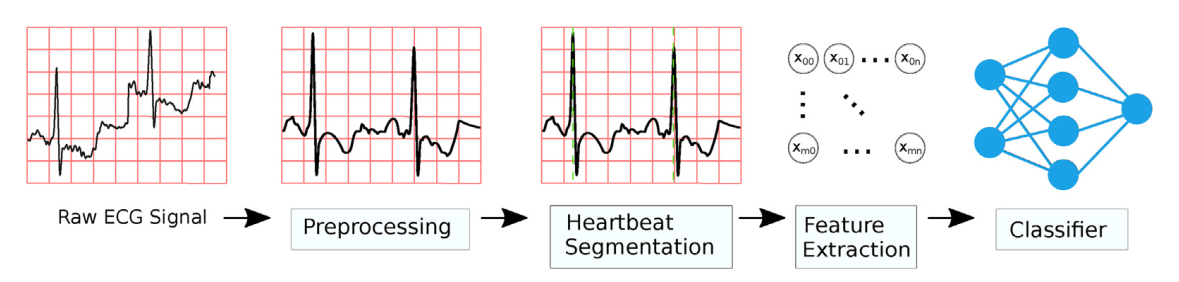
\includegraphics[width=15cm]{Figures/classifier.png}
\caption{مراحل اصلی یک سیستم خودکار تشخیص آریتمی\cite{Mondejar}}
\label{fig:classifierPicture}
\end{figure}

در این پروژه، هدف بر این است که بستری بی‌درنگ برای تشخیص آریتمی فراهم شود. به دلیل اهمیت تشخیص سریع در برخی از انواع خطرناک آریتمی، به خصوص آریتمی‌هایی که منجر به ایست ناگهانی قلبی می‌شوند، بی‌درنگ بودن این سیستم حایز اهمیت است. این امر نیازمند این است که تمامی بخش‌های سیستم، شامل بخش پیش‌پردازش،‌ بخش استخراج ویژگی و الگوریتم دسته‌بندی، همگی توانایی کارکردن به صورت برخط را داشته‌باشند. به بیان دیگر این سیستم به شکل خط‌لوله‌ای طراحی شده‌است که در آن ضربان‌ها به صورت پی‌در‌پی تولید، پردازش‌ و دسته‌بندی می‌شوند. پس از پیاده‌سازی، تاخیر هر یک از بخش‌ها اندازه‌گیری شده و تاخیر کلی سیستم تخمین زده می‌شود. 
همان‌طور که گفته‌شد، اولین بخش سیستم، بخش پیش‌پردازش ضربان قلب است. در این بخش یک الگوریتم تشخیص QRS طبق روش پن و تامپکینز (منبع)  پیاده‌سازی شده‌است. این الگوریتم یک روش بی‌درنگ است که سیگنال دیجیتال‌شده‌ی نوار قلب را به عنوان ورودی دریافت کرده و موقعیت زمانی قله‌های R را در هر یک از ضربان‌ها تشخیص می‌دهد. فاصله‌ی هر قله‌ی R تشخیص‌داده‌شده با قله‌ی بعدی و قبلی خود، که تحت عنوان فاصله‌ی R-R شناخته می‌شود، مهم‌ترین ویژگی در تشخیص نوع ضربان قلب (نوع آریتمی آن ضربان) است. (نیازمند منبع) 
در مرحله‌ی بعد، ویژگی‌های مورد نظر، از فواصل R-R تشخیص‌داده‌شده استخراج می‌گردند. این ویژگی‌ها سپس به یک دسته‌بند SVM که پیش‌تر مراحل یادگیری را طی کرده‌است، داده می‌شوند و دسته‌بند به کمک ویژگی‌های ورودی، نوع آریتمی را تشخیص می‌دهد. ضربان‌های دارای آریتمی انواع متعددی دارند که در ۵ دسته‌ی کلی دسته‌بندی می‌شوند. خروجی سیستم ما، تشخیص یکی از این دسته‌ها برای هر ضربان قلب است.

یکی از نیازمندی‌های بستر طراحی‌شده در این پروژه، این است که بتوان سیستمی قابل حمل و قابل استفاده‌ی آسان برای بیمار را بر روی این بستر پیاده‌سازی کرد. برای پیاده‌سازی این کاربرد، اینترنت اشیا راه‌حل مناسبی تشخیص داده‌شد. در چنین کاربردی، انتظار می‌رود بیمار دستگاهی ساده در اختیار داشته‌باشد که ضربان قلب او را دریافت کرده و پیش‌پردازش‌هایی ساده را بر روی آن پیاده نماید، و پردازش‌های پیچیده‌تر برای تشخیص آریتمی، بر عهده‌ی یک سرور با توان پردازشی بالاتری باشد. سپس نتایج این پردازش‌ها به اطلاع بیمار و پزشک او برسد.

 برای این منظور، معماری کلی سیستم به دو بخش تقسیم شد. بخش اول سیستم، وظیفه‌ی دریافت ضربان قلب از بیمار،‌ انجام پیش‌پردازش‌هایی بر روی آن، و در انتها ارسال نتایج پیش‌پردازش به سرور را دارد. این بخش به صورت سخت‌افزاری پیاده شده‌است و کافی است یک حس‌گر دیجیتال ضربان قلب، برای دریافت ضربان قلب بیمار به آن متصل شود. 
بخش دوم سیستم با استفاده از الگوریتم‌های یادگیری ماشین، و بر روی یک سرور پیاده‌سازی شده‌است. در این سرور، نتایج پیش‌پردازش‌های انجام شده در بخش قبل در سرور دریافت شده و ویژگی‌های هر ضربان استخراج می‌شود. سپس با استفاده از این ویژگی‌ها، عمل دسته‌بندی ضربان‌ها انجام می‌شود.

کارهای گذشته در قسمت فیچر:
در کارهای گذشته، ویژگی‌های مختلفی برای توصیف ضربان قلب معرفی شده‌اند. تبدیل موجک (منبع) و آمارهای مرتبه بالاتر (HOS) (منبع) از جمله‌ی این ویژگی‌ها هستند. در تبدیل موجک، اطلاعاتی هم در حوزه‌ی زمان و هم در حوزه‌ی فرکانس از سیگنال استخراج می‌شود. 
(توضیحات بیشتر در مورد اینترنت اشیا)
در برخی از پژوهش‌ها از بازه‌های R-R به عنوان ویژگی استفاده شده‌است (منبع) (منبع ۶۷ تا ۷۹ سوروی). آریتمی قلبی باعث برهم‌خوردن آهنگ تپش و در نتیجه‌ی آن، توازن منحنی ضربان قلب می‌شود، و ابن اتفاق تاثیر مستقیمی بر روی نوسانات فاصله‌های قله‌های R می‌گذارد. (منبع ۱ سوروی) به همین دلیل ویژگی R-R ظرفیت بالایی برای تشخیص انواع آریتمی دارد. این ویژگی در بین ویژگی‌های به کار گرفته‌شده پراستفاده‌ترین است. (منبع ۱۵ مرده خوار)
این ویژگی، نسبت به ویژگی‌های morphological حجم کم‌تری به خود اختصاص می‌دهد. در کار پیش رو، ویژگی‌های استخراج شده از ضربان قلب بیمار در مرحله‌ی پیش‌پردازش، به یک سرور فرستاده می‌شوند تا پردازش‌های بیش‌تر بر روی آن‌ها انجام شود. از این رو لازم است حجم داده‌های ارسال‌شده، و پیرو آن، حجم ویژگی‌های استخراج‌شده کنترل شود. در صورتی که ویژگی‌های استخراج‌شده حجم زیادی داشته‌باشند، تاخیر ارسال آن‌ها به سرور بالا رفته و تاثیری منفی بر روی تاخیر کل سیستم خواهدداشت. با توجه به اهمیت تاخیر پایین و بی‌درنگ بودن عملیات در این کاربرد، و همچنین دقت بالای بازه‌های R-R در تعیین نوع آریتمی، از این ویژگی استفاده کردیم. 
(normalized RR)

قدم بعد، پیاده‌سازی یک دسته‌بند برای تعیین نوع آریتمی است. در کارهای گذشته از الگوریتم‌های دسته‌بندی مانند SVM ANN (از رو مقاله هه بنویس با منبع) استفاده شده‌است. در کار پیش رو، SVM به دلیل کارایی مناسبی که در کارهای گذشته (منبع ۲۱ و ۲۲ مرده خوار) نشان داده‌است به کار گرفته شده‌است. 



%---------------------- begin chap 2 -------------
\cchapter{مفاهیم اولیه}
\label{chap:lit}
\pagebreak

\section {قلب و نحوه‌ی عملکرد آن}
قلب ماهیچه‌ای متشکل از ۴ حفره است. دو حفره‌ی بالایی، دهلیزهای چپ و راست نامیده می‌شوند و دو حفره‌ی پایینی، بطن‌های چپ و راست نام دارند. در هر سیکل تپش قلب، خونِ بدون اکسیژن از طریق بزرگ‌سیاهرگ‌های بالایی و پایینی وارد دهلیز راست می‌شود. پس از طی فرایندی در قلب، خون دارای اکسیژن شده و از بطن چپ خارج می‌شود. این خون سپس از طریق سرخرگ‌ها به اعضای بدن می‌رسد. قلب یک فرد بزرگسال سالم، به طور متوسط بین ۶۰ تا ۱۰۰ بار در دقیقه می‌تپد. \cite{MayoClinic}

عملکرد قلب توسط یک سیستم الکتریکی و به وسیله‌ی سیگنال‌های تولید شده در آن کنترل می‌شود. این سیگنال‌ها دیواره‌های قلب را تحریک می‌کنند و با انقباض دیواره‌ها، خون از قلب خارج شده و در سیستم گردش خون جریان می‌یابد. در ادامه به طور دقیق به نحوه‌ی عملکرد قلب می‌پردازیم. 


\subsection {سیستم هدایت الکتریکی قلب}
تمامی فعالیت‌های قلب که منجر به پمپ‌کردن خون در بدن می‌شوند، تحت کنترل سیستم هدایت الکتریکی قلب \LTRfootnote{Cardiac conduction system} قرار دارند. این سیستم با انتقال الکتریکی سیگنال‌های تولید شده، باعث به تپش درآمدن ماهیچه‌ی قلب می‌شود. بخش‌های اصلی این سیستم عبارت اند از:

\begin{enumerate}
	\item گره سینوسی‌دهلیزی \LTRfootnote{Sinoatrial node} \lr{(SA)} در دهلیز 
	راست قلب
	\item گره دهلیزی‌بطنی \LTRfootnote{Atrioventricular node} \lr{(AV)} در سپتوم داخل‌دهلیزی قلب \LTRfootnote {Interatrial septum} (دیواره‌ای ماهیچه‌ای که دهلیز راست و چپ قلب را جدا می‌کند)
	\item سیستم هیس-پورکینژ \LTRfootnote{His-Purkinje system} در دیواره‌های بطن‌های قلب
\end{enumerate}
این بخش‌ها در شکل \ref{fig:conduction} قابل مشاهده هستند.

\begin{figure}
\centering
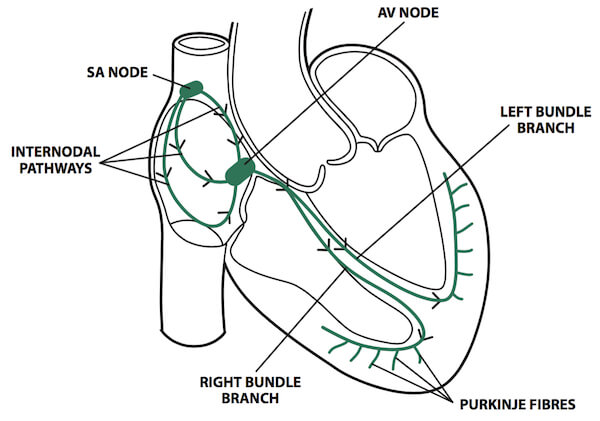
\includegraphics[width=12cm]{Figures/conduction.jpg}
\caption{سیستم هدایت الکتریکی قلب\cite{Medicalexamprep}}
\label{fig:conduction}
\end{figure}

نقطه‌ی آغاز هر ضربان قلب، گره سینوسی‌دهلیزی است. این گره با تولید سیگنالی هر دو دهلیز را تحریک به انقباض می‌کند و در نتیجه‌ی این عمل، خون از طریق دریچه‌های باز، از دو دهلیز وارد دو بطن قلب می‌شود. سپس سیگنال وارد گره دهلیزی‌بطنی شده و برای لحظه‌ای کوتاه تاخیر می‌کند، تا خون فرصت پر کردن دو بطن قلب را پیدا کند. 

در مرحله‌ی بعد، سیگنال آزاد شده و در مسیری به نام دسته‌ی هیس \LTRfootnote{Hiss bundle} واقع در دیواره‌های بطن‌ها حرکت خود را ادامه می‌دهد. در این مرحله، سیگنال به دو دسته تقسیم شده و این دو دسته از طریق دو مسیر به نام‌های فیبرهای پورکینژ \LTRfootnote{Purkinje fibers} چپ و راست، به ترتیب وارد بطن چپ و راست قلب می‌شوند. این عمل باعث انقباض دو بطن می‌شود و در نتیجه‌ی این عمل، خون از طریق دریچه‌های بیرونی قلب، از آن خارج شده و به ریه‌ها و بقیه‌ی اعضای بدن انتقال می‌یابد. در این مرحله سیگنال از بطن‌ها گذر می‌کند و دو بطن وارد حالت استراحت می‌شوند، تا سیگنال بعدی فرابرسد.

تولید پی‌در‌پی این سیگنال‌ها، باعث انقباض و استراحت منظم و هماهنگ قلب شده و ضربان قلب را ایجاد می‌کند. در واقع ضربان قلب هر شخص، توسط تعداد دفعاتی در طول یک دقیقه که گره سینوسی‌دهلیزی سیگنال تولید می‌کند تعیین می‌شود. \cite{Heart} 


\section{آریتمی قلبی}
آریتمی قلبی به دسته‌ای از بیماری‌های قلبی اطلاق می‌شود که در آن‌ها، آهنگ تپش قلب حالتی غیرعادی پیدا می‌کند. به طور کلی دلیل رخ دادن آریتمی، عدم انتقال درست سیگنال‌های الکتریکی قلب بیان می‌شود. تعدادی از انواع آریتمی‌ها می‌توانند شدیدا خطرناک و کشنده باشند. اکثر آریتمی‌ها بی خطر شناخته شده‌اند، اما در صورت عدم تشخیص و رسیدگی به موقع می‌توانند زندگی عادی فرد مبتلا را آشفته ساخته یا حیات او را تهدید کنند. 
\subsection{انواع آریتمی قلبی}
آریتمی‌ها بر اساس نوع اختلالی که در ضربان قلب ایجاد می‌کنند، به چهار دسته‌ی کلی تقسیم می‌شوند.
\begin{enumerate}
	\item ضربان‌های زودرس \LTRfootnote{Premature beats}: در این دسته از آریتمی‌ها، قلب ضربا‌ن‌هایی زودرس تولید می‌کند که آهنگ طبیعی تپش آن را مختل می‌کنند. در صورتی که ضربان زودرس در بطن قلب تولید شده‌باشد، ضربان زودرس بطنی\LTRfootnote{Premature Ventricular Complex (PVC)}، و در صورتی که در دهلیز ایجاد شده باشد، ضربان زودرس دهلیزی \LTRfootnote{Premature Atrial Complex (AVC)} نامیده می‌شود.
	\item تاکی‌کاردی فوق بطنی \LTRfootnote{Supraventricular Tachycardia (SVT)}: در این نوع آریتمی، قلب به صورتی غیرعادی تندتر از معمول  (تقریبا بیش از ۱۰۰ ضربان در دقیقه) می‌تپد. \cite{Amboss} این آریتمی‌ها در بین گره سینوسی‌دهلیزی و گره دهلیزی‌بطنی ایجاد می‌شوند. 
	\item آریتمی‌های بطنی \LTRfootnote {Ventricular arrhythmia}:  آریتمی‌هایی که از پایین گره دهلیزی‌بطنی (در سطح بطن قلب) ریشه می‌گیرند در این دسته قرار دارند.
	\item برادی‌کاردی \LTRfootnote{Bradycardia}: در این نوع آریتمی، قلب بیمار آرام‌تر از حالت عادی می‌تپد و نرخ ضربان قلب معمولا پایین‌تر از ۶۰ تپش در دقیقه است.  \cite{Verywellhealth}

\end{enumerate}

\section{سیگنال نوار قلب}
همان طور که گفته شد، سلول‌های گره سینوسی تحریک الکتریکی منظمی را ایجاد می‌کنند که توسط سیستم هدایت الکتریکی موجود در قلب، به بخش‌های دیگر آن انتشار یافته و باعث تپش متناوب قلب می‌شود. نتیجه‌ی این فعالیت، ایجاد جریان الکتریکی در سطح بدن و تحریک تغییرات در پتانسیل الکتریکی سطح پوست است. این سیگنال‌ها را می‌توان به وسیله‌ی الکترودها و دیگر تجهیزات، ثبت و اندازه‌گیری نمود.

در فرایند ثبت نوار قلب، اختلاف پتانسیل بین نقاط قرارگیری الکترودها بر روی بدن اندازه‌گیری شده و معمولا به کمک تقویت‌کننده‌های عملیاتی \LTRfootnote{Operational amplifiers} بهبود داده می‌شود. در مرحله‌ی بعد، سیگنال ابتدا از یک فیلتر بالاگذر و سپس از یک فیلتر پایین‌گذر تصحیح فرکانس عبور داده‌می‌شود. در نهایت این سیگنال آنالوگ، به سیگنال دیجیتال تبدیل می‌شود. منحنی گرافیکی رسم شده در انتهای این فرایند، نوار قلب، و یا به اختصار \lr{ECG} نامیده می‌شود. 

امروزه در روش‌های استاندارد اندازه‌گیری نوار قلب،تعدادی الکترود بر روی سطح پوست قرارمی‌گیرند و یکی از آن‌ها به عنوان مرجع \LTRfootnote{Reference} برای دیگر الکترودها در نظر گرفته می‌شود. به طور معمول، الکترود مرجع روی ساق پای راست نصب می‌شود. \cite{ECGSurvey} هر یک از الکترودهای دیگر، ولتاژ ناحیه‌ی قرارگیری خود را نسبت به ولتاژ الکترود مرجع اندازه‌گیری می‌کنند. هر یک از این اختلاف پتانسیل‌های اندازه‌گیری شده، یک لید \LTRfootnote{Lead} نامیده می‌شود. 
\subsection{نحوه‌ی قرارگیری الکترودها بر روی پوست و لیدهای تولیدشده}

یکی از ترکیب‌های رایج قراردادن الکترودها متشکل از ۱۰ الکترود است که بر روی دست، پا و سینه‌ی بیمار قرار می‌گیرند. از ترکیب این الکترودها ۱۲ لید ایجاد می‌شود که به سه دسته‌ی کلی تقسیم می‌شوند:
\begin{itemize}
	\item  سه لید دوقطبی اندامی \LTRfootnote{Bipolar limb leads} به نام‌های \lr{I}، \lr{II} و \lr{III}
	\item سه لید تک‌قطبی اندامی \LTRfootnote{Unipolar limb leads} به نام‌های \lr{aVF}، \lr{aVL} و \lr{aVR}
	\item شش لید تک‌قطبی سینه‌ای به نام‌های \lr{V1} تا \lr{V6}
\end{itemize}
  هر یک از این لیدها فعالیت الکتریکی قلب را از یک زاویه‌ی خاص در بدن نشان می‌دهد. پرکاربردترین لید برای تشخیص بیماری‌های قلبی، لید \lr{II} می‌باشد که اختلاف پتانسیل بین الکترودهای ساق پای چپ و بازوی راست را نشان می‌دهد. در شکل \ref{fig:leads} یک نوار قلب ۱۲ لیدی مشاهده می‌شود. منحنی رسم شده از هر لید به صورت جداگانه نشان داده شده‌است و لید \lr{II} نیز به تنهایی رسم شده‌است. این لید به خصوص از آن جهت اهمیت دارد که نمای خوبی از ترکیب \lr{QRS}
ارائه می‌دهد. در بخش بعد در مورد این موضوع به تفصیل توضیح داده خواهد شد.
\begin{figure}
\centering
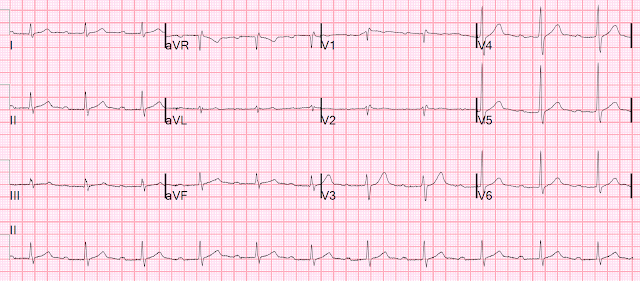
\includegraphics[width=16cm]{Figures/leads.png}
\caption{نوار قلب ۱۲ لیدی گرفته‌شده از یک فرد سالم\cite{Drsmith}}
\label{fig:leads}
\end{figure}

\subsection{ترکیب QRS}
با بررسی یک سیکل ضربان قلب در نوار قلب، ۵ انحراف\LTRfootnote{Deflection}
یا موج پراهمیت دیده می‌شود. اولین موج، \lr{P} نام دارد که با فعال شدن دهلیزهای راست و چپ و بالارفتن پتانسیل الکتریکی آن‌ها اتفاق می‌افتد. سه موج بعدی به ترتیب \lr{Q}، \lr{R} و \lr{S} نام دارند. این سه موج به ترتیب و با فاصله‌ی کمی از هم رخ می‌دهند و عموما به عنوان یک ترکیب، همراه یکدیگر بررسی می‌شوند. این ترکیب که \lr{QRS} نامیده می‌شود، واضح‌ترین بخش مشاهده‌شده در یک سیکل قلبی است که مدت زمان بالارفتن پتانسیل ماهیچه‌های بطنی قلب را نشان می‌دهد. موج بعدی \lr{T} نام دارد که در طول آن بطن‌ها منقبض شده و بار مثبت خود را تخلیه می‌کنند. ترکیب \lr{QRS} در شکل \ref{fig:QRS} مشاهده می‌شود.

\begin{figure}
\centering
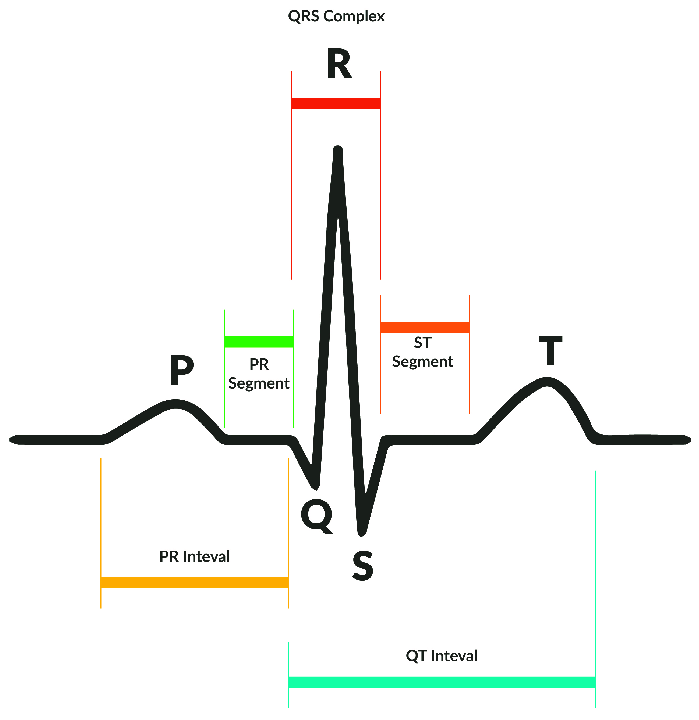
\includegraphics[width=10cm]{Figures/qrs.png}
\caption{ ترکیب \lr{QRS} \cite{Miramontes2017}}
\label{fig:QRS}
\end{figure}
 
\subsubsection{بازه‌های زمانی مهم در سیکل ضربان قلب}
مهم‌ترین بازه‌های زمانی در یک سیکل ضربان قلب عبارت اند از:
\begin{itemize}
	\item بازه‌ی \lr{PR}: فاصله‌ی زمانی از ابتدای موج \lr{P} تا ابتدای ترکیب QRS 
	\item مدت‌زمان \lr{QRS}: مدت‌زمان رخ‌دادن ترکیب \lr{QRS}
	\item بازه‌ی \lr{QT}: فاصله‌ی زمانی از ابتدای ترکیب \lr{QRS} تا انتهای موج \lr{T}
	\item بازه‌ی \lr{RR}: مدت‌زمان سیکل کامل قلب که نشان‌دهنده‌ی سیکل کامل بطن‌ها می‌باشد. 
	\item بازه‌ی \lr{PP}: مدت‌زمان سیکل کامل دهلیزی
\end{itemize}


 \subsubsection{تاثیر آریتمی قلبی بر روی شکل ترکیب QRS}
 وجود آریتمی قلبی می‌تواند باعث تغییر شدید در امواج \lr{Q}، \lr{R} و \lr{S} شود. لید \lr{II} به دلیل واضح‌تر نشان دادن ترکیب \lr{QRS} و لیدهای \lr{V1} تا \lr{V6} به دلیل این که الکترودهای آن‌ها بر روی سینه قرارگرفته و تشخیص بهتر تغییرات پتانسیل ماهیچه‌ی بطنی را ممکن می‌سازند، تا کنون بهترین نتایج را در تشخیص آریتمی نشان داده‌اند. \cite{ECGSurvey}

در طول بازه‌ی زمانی \lr{QRS} بطن‌هابه وسیله‌ی سیستم هیس-پورکینژ منقبض می‌شوند. این سیستم شامل سلول‌هایی در دیواره‌های بطن‌ها است که خاصیت رسانایی سریع الکتریکی را دارند. در صورت ایجاد اختلال در کار این سیستم و ضعیف‌شدن خاصیت رسانایی الکتریکی سلول‌ها، بازه‌ی زمانی \lr{QRS} طولانی‌تر می‌شود. در برخی موارد سیگنال الکتریکی به جای انتقال یافتن از طریق سیستم هیس-پورکینژ، از طریق ماهیچه‌های قلب منتقل می‌شود. این اتفاق منجر به طولانی شدن زمان انتقال الکتریکی سیگنال و در نتیجه عریض شدن بازه‌ی \lr{QRS} می‌شود.
 به طور معمول طول یک بازه‌ی \lr{QRS} بین ۰/۰۸ تا ۰/۱ ثانیه است. در مواردی که طول این بازه از ۰/۱۲ ثانیه بیشتر شود، \lr{QRS} غیرعادی تلقی می‌شود. \cite{Healio}

\section{مسائل دسته‌بندی}

در مسائل دسته‌بندی، ورودی‌های مسئله تعدادی داده هستند و مطلوب مسئله، جای دادن هر یک از داده‌ها در یک دسته یا کلاس است. به بیان رسمی‌تر در این مسئله‌ها، هدف، تخمین‌زدن یک نگاشت از متغیرهای ورودی \lr{X} به تعدادی متغیر خروجی گسسته \lr{Y} است. این متغیرهای خروجی تعدادی برچسب\LTRfootnote{Label} هستند که تعیین می‌کنند هر داده در کدام دسته قرار می‌گیرد. تعداد این دسته‌ها می‌تواند دو و یا بیشتر باشد که در حالت دوم، مسئله یک مسئله‌ی دسته‌بندی چنددسته‌ای\LTRfootnote{Multiclass classification problem} نامیده می‌شود. 

\subsection{روش ماشین بردار پشتیبانی (SVM)}
یکی از پرکاربردترین دسته‌های الگوریتم برای حل مسایل دسته‌بندی، الگوریتم‌های \lr{SVM} هستند. در این الگوریتم‌ها، داده‌ها به مثابه‌ی نقطه‌هایی در یک فضای \lr{N}بعدی فرض می‌شوند. هدف الگوریتم، یافتن ابرصفحه‌هایی\LTRfootnote{Hyperplanes} است که به طور بهینه نقطه‌های داده‌ها را به کلاس‌های متعدد دسته‌بندی کند. تعداد بعدهای این فضا \lr{(N)} برابر با تعداد ویژگی‌ها است. معمولا تعداد زیادی ابرصفحه را می‌توان برای جداسازی دو کلاس مختلف از داده‌ها یافت، اما در این الگوریتم، هدف یافتن ابرصفحه‌ای است که بیشترین فاصله را با نزدیک‌ترین نقطه‌ی داده در هر یک از کلاس‌ها داشته‌باشد. این فاصله، حاشیه\LTRfootnote{Margin} نامیده می‌شود. 

\subsubsection{ابرصفحه}
ابرصفحه مرزی است که نقاط داده‌ها را در یک فضای \lr{N}بعدی به دو بخش تقسیم می‌کند. برای مثال در مسئله‌ای با دو کلاس هدف، نقاطی که در هر یک از دو سمت ابرصفحه‌ی به‌دست‌آمده قرار می‌گیرند، به یکی از آن دو کلاس تعلق می‌یابند. تعداد بعد ابرصفحه بسته به تعداد ویژگی‌های داده‌ها است. مثلا در مسئله‌ای که سه ویژگی برای داده‌ها به دست آورده‌ایم، فضای داده ۳بعدی بوده و در نتیجه ابرصفحه‌ی جداکننده‌ی داده‌ها نیز ۳بعدی خواهد بود.

\subsubsection{بردار پشتیبانی}
بردارهای پشتیبانی، نقاط داده‌ای هستند که ابرصفحه را تعریف می‌کنند. این نقاط به ابرصفحه نزدیک‌تر بوده و بر روی موقعیت قرارگیری و جهت آن تاثیر می‌گذارند. به کمک این بردارها، ابرصفحه‌ای با بیشترین حاشیه برای دسته‌بندی انتخاب می‌شود.\cite{SVM} نمودار یک مسئله‌ی دسته‌بندی دوبعدی در شکل \ref{fig:SVMClassification} دیده می‌شود.

\begin{figure}
\centering
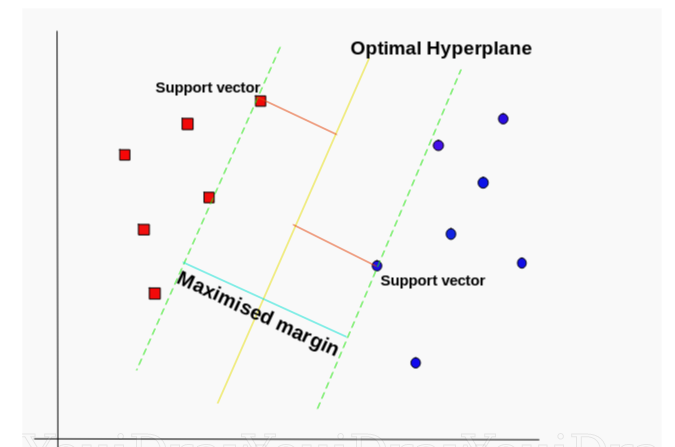
\includegraphics[width=10cm]{Figures/svmMargin.png}
\caption{ نموداری از حل یک مسئله‌ی دسته‌بندی دوبعدی با روش \lr{SVM}\cite{SVM}}
\label{fig:SVMClassification}
\end{figure}
 

\subsubsection{ تابع کرنل}
در روش \lr{SVM} برای دسته‌بندی داده‌ها از توابعی به نام توابع کرنل استفاده می‌شود. تابع کرنل داده را به عنوان ورودی گرفته و آن را به فضایی دیگر انتقال \LTRfootnote{Transform} می‌دهد. به کمک تابع کرنل، داده‌هایی که در فضای عادی مشاهده شده‌اند، به فضایی با تعداد ابعاد بالاتر انتقال می‌یابند که در چنین فضایی امکان جداسازی آن‌ها وجود دارد. در واقع هر مدل خطی را می‌توان به کمک تابع کرنل به یک مدل غیر خطی تبدیل کرد، به این صورت که ویژگی‌های مدل را با یک تابع کرنل جایگزین کنیم. 

به طور رسمی‌تر می‌توان تابع کرنل را به این صورت تعریف کرد: به ازای هر  $x$  و $x'$ در فضای $X$ می‌توان توابعی به صورت $k(x, x')$ را یافت که حاصل ضرب داخلی دو نقطه در فضای دیگری به نام $V$ است. این روابط در معادله‌ی \ref{eq:kernel} قابل مشاهده است.\cite{KernelSVM} 

\begin{equation}
\begin{split}
	& k: X \times X \to \mathbb{R} \\
	& k(x_i, x_j) = \bigg \langle \Phi (X_i), \Phi(X_j) \bigg \rangle
\end{split}
\label{eq:kernel}
\end{equation}

ساده‌ترین نوع کرنل، کرنل خطی است. این توابع  داده‌ها را به فضایی با تعداد بعد بالاتر نگاشت نمی‌کنند، به همین دلیل بهتر است در مسائلی که داده‌ها به صورت خطی قابل جداسازی هستند، از این نوع کرنل استفاده شود. 
 این نوع کرنل‌ها به دلیل سادگی و خطی بودن، سرعت بیشتری در دسته‌بندی دارند. معمولا در مسائلی که تعداد ویژگی‌ها زیاد بوده و نگاشت داده‌ها به نقاطی در فضای با تعداد بعدهای بالاتر تاثیر چشمگیری در بهبود دسته‌بندی ندارد، از کرنل خطی استفاده می‌شود. \cite{LinearSVM} 
 نوع پیچیده‌تری از کرنل که در بسیاری از مسائل دسته‌بندی کاربرد دارد. کرنل \lr{RBF}\LTRfootnote{ Radial Basis Function} نام دارد. این تابع بر روی نقطه‌ی $X_i$ و $X_j$ در فضای $X$ که یک فضای ورودی است در معادله‌ی \ref{eq:kernelRBF} قابل مشاهده است.\cite{kernelRBF}
   
\begin{equation}
	 k(X_i, X_j) = \exp(-\frac{{||X_i-X_j||}^2}{2\sigma^2})
\label{eq:kernelRBF}
\end{equation}
در این رابطه $\sigma$ یک پارامتر آزاد است. این تابع، دو بردار $X_i$  و $X_j$ که در فضایی دو بعدی قرار دارند را به یک بردار بی‌نهایت نگاشت می‌کند. این عمل باعث می‌شود نقاط داده به نقاطی در فضایی با تعداد بعد بیشتر نگاشت شوند. در مسائلی که در فضای اصلی داده‌های ورودی، ابرصفحه‌ای برای جداسازی کلاس‌ها یافت نمی‌شود، می‌توان با استفاده از کرنل \lr{RBF} در فضایی با تعداد بعد بالاتر، ابرصفحه‌ای برای جداسازی کلاس‌ها یافت. این موضوع در شکل \ref{fig:RBFKernel} قابل مشاهده است. این نوع تابع کرنل، زمان و قدرت پردازشی بیشتری به نسبت کرنل خطی مصرف می‌کند.

\begin{figure}
\centering
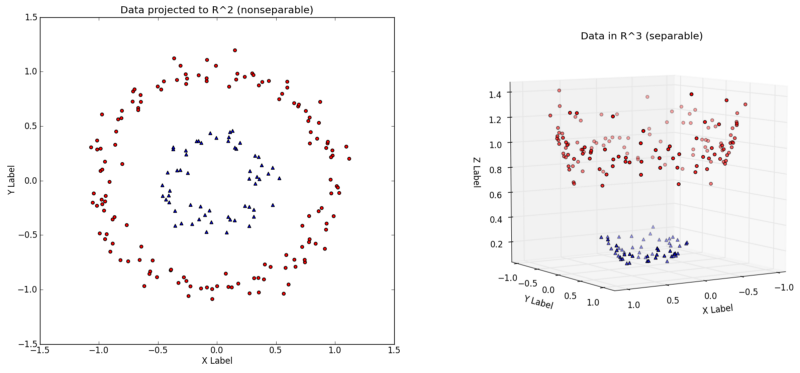
\includegraphics[width=15cm]{Figures/RBFKernel.png}
\caption{ سمت چپ: داده‌های غیر قابل جداسازی توسط یک ابرصفحه در یک فضای دوبعدی، سمت راست: داده‌های انتقال‌داده‌شده به فضای سه‌بعدی و قابل جداسازی\cite{TowardsScienceRBF}}
\label{fig:SVMClassification}
\end{figure}

\subsubsection{ انجام دسته‌بندی  با استفاده از تابع کرنل RBF}
برای انجام عمل دسته‌بندی با استفاده از کرنل \lr{RBF}، لازم است تعدادی پارامتر برای این تابع تعیین شوند. میزان تاثیر هر یک از این پارامترها بر روی نتیجه‌ی نهایی دسته‌بندی معمولا به کاربرد وابسته است. در ادامه تعدادی از  مهم‌ترین پارامترها توضیح داده می شوند. 
\begin{itemize}
	\item پارامتر $\gamma$:
	\\
	$\gamma$ پارامتر آزادی است که در تابع کرنل \lr{RBF} وجود دارد. این پارامتر تعیین می‌کند یک داده به تنهایی چقدر می‌تواند بر روی نتیجه‌ی نهایی دسته‌بندی تاثیر داشته‌باشد. در صورت کوچک‌بودن $\gamma$ این تاثیر زیاد و در صورت بزرگ‌بودن آن، این تاثیر کم است. این پارامتر را می‌توان به صورت عکس شعاع تاثیر نمونه‌هایی که مدل به عنوان بردار ساپورت انتخاب می‌کند دانست. گامای کوچک باعث می‌شود منحنی گاوسی تابع کرنل، واریانس زیادی داشته‌باشد. اگر $X_j$ یک بردار ساپورت باشد، کوچک‌بودن $\gamma$ نتیجه می‌دهد که کلاس این بردار ساپورت، بر روی تشخیص کلاس $X_i$  تاثیر دارد حتی اگر فاصله‌ی آن‌ها زیاد باشد. برعکس اگر $\gamma$ بزرگ باشد، واریانس کوچک بوده و این نتیجه می‌دهد یک بردار ساپورت تاثیر زیادی بر روی تشخیص کلاس نمونه‌ها ندارد.

رفتار مدل نسبت به مقدار $\gamma$ بسیار حساس است. به طور کلی می‌توان گفت بزرگ‌بودن بیش از حد $\gamma$ باعث می‌شود شعاع ناحیه‌ای که بردار ساپورت بر روی آن تاثیر دارد بسیار کوچک شده و تنها خود بردار را در بر بگیرد. کوچک‌بودن بیش از حد آن نیز باعث می‌شود ناحیه‌ی تاثیر هر یک از بردارهای ساپورت به اندازه‌ی کل مجموعه‌ی داده‌ها بزرگ می‌شود و مدل نهایی تفاوتی با یک کرنل خطی که در آن تعدادی ابرصفحه نقاط داده را از هم جدا می‌کنند نخواهد داشت.

	\item پارامتر $C$:
	\\
	در \lr{SVM} هدف پیدا کردن مرز جداکننده‌ای است که تمامی داده‌های مربوط به هر یک از کلاس‌ها را به درستی جدا کند. در صورت وجود خطا در نمونه‌ها و یا داده‌های غیرعادی، این کار باعث می‌شود مدل نتواند مرز مناسبی برای جداسازی کلاس‌ها بیابد. به همین علت مفهوم حاشیه‌ی نرم\LTRfootnote{Soft margin} مطرح می‌شود. با اعمال حاشیه‌ی نرم، به \lr{SVM} اجازه داده می‌شود برخی از نمونه‌ها را در دسته‌بندی در نظر نگیرد و برخی از نمونه‌ها را در کلاس نادرست دسته‌بندی کند. پارامتر $C$ شدت این عمل را کنترل می‌کند. این پارامتر تاثیر هر یک از بردارهای ساپورت بر روی حاشیه‌ی ابرصفحه‌ی جدا کننده را نشان می‌دهد. مدلی با $C$ پایین‌تر، آسان‌گیرانه تر دسته‌بندی کرده و منجر به داشتن داده‌های بیشتری با دسته‌بندی نادرست می‌شود، اما در عوض حاشیه‌ی بالاتری را نتیجه می‌دهد. 
\end{itemize} 
 

\subsection{دسته‌بندی داده‌ها با استفاده از روش SVM}
روش کلی ساخت یک مدل \lr{SVM} به این صورت است که داده‌ها را به دو مجموعه‌ی داده‌های آموزشی\LTRfootnote{Training data set} و داده‌های تست\LTRfootnote{Test data set} تقسیم می‌کنیم. نحوه‌ی تقسیم داده‌ها به این دو مجموعه تا حد زیادی به مسئله وابسته است. نحوه‌ی کلی انجام دسته‌بندی به این صورت است که ابتدا عملیات آموزش بر روی مجموعه‌ی اول انجام شده و مدل SVM ساخته می‌شود. سپس این مدل بر روی محموعه‌ی تست آزموده شده و دقت دسته‌بندی، با توجه به معیارهای کارایی مورد نظر در مسئله اندازه‌گیری می‌شود.

%------------------------ Start chapter 3 -------------
\cchapter{روش حل مسئله}
\pagebreak

\section{مقدمه}
 این پروژه در دو بخش کلی پیش‌پردازش در سمت سخت‌افزار و پردازش در سرور انجام شده‌است. در بخش اول، تعدادی پردازش اولیه بر روی داده‌های خام ضربان قلب انجام می‌شود. این بخش یک بستر پیاده شده بر روی سخت‌افزار است که برای کامل شدن باید به یک سنسور ضربان قلب متصل شود. این بخش همراه بیمار خواهد بود و پردازش‌های ساده‌ی اولیه را بر روی سیگنال نوار قلب انجام داده و نتایج را به سرور ارسال می‌کند.  پردازش‌های پیچیده‌تر برای تشخیص آریتمی بر عهده‌ی سرور خواهد بود. در سرور یک الگوریتم دسته‌بندی بر روی داده‌ها انجام شده و کلاس آریتمی آن‌ها تشخیص داده می‌شود.

\section{عملیات پیش‌پردازش بر روی سخت‌افزار} 
در این بخش عملیات پیش‌پردازش با هدف تشخیص ترکیب \lr{QRS} در هر ضربان قلب بر روی سیگنال دیجیتال ضربان قلب اجرا می‌شود. خروجی این عملیات، موقعیت زمانی قله‌ی \lr{R} در ترکیب \lr{QRS} هر ضربان است که در پردازش‌های آینده برای تشخیص آریتمی آن ضربان مورد استفاده قرار می‌گیرد. این بخش بر روی یک ماژول \lr{ESP8266} که یک ماژول وای‌فای دارای یک پردازنده‌ی ۸۰ مگاهرتزی است، پیاده‌سازی می‌شود. این ماژول علاوه بر انجام پیش‌پردازش، ارسال داده‌‌های حاصل از آن از طریق وای‌فای را نیز بر عهده دارد. قسمت‌های پیاده‌سازی‌شده در این بخش در شکل \ref{fig:preprocessing} در کادر مشخص شده‌اند.
\begin{figure}[!htb]
\centering
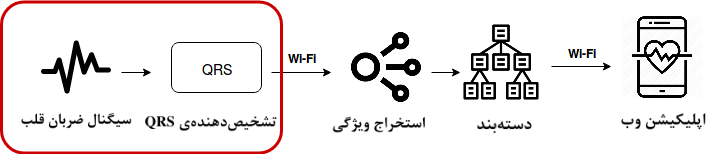
\includegraphics[width=16cm]{Figures/preprocessing.png}
\caption{بخش پیش‌پردازش بر روی سخت‌افزار در مراحل تشخیص آریتمی}
\label{fig:preprocessing}
\end{figure}

	\subsection{مراحل تشخیص QRS}

همان‌طور که گفته شد، تشخیص \lr{QRS} با استفاده از الگوریتم پن-تامپکینز صورت می‌گیرد. مراحل کلی این الگوریتم در شکل \ref{fig:qrsPan} نشان داده شده‌است. در این فرایند، پیش از ورود سیگنال نوار قلب به ماژول پیش‌پردازش، نوار قلب خام گرفته‌شده از بیمار  از یک مبدل آنالوگ به دیجیتال\LTRfootnote{ADC} عبور کرده و با نرخ نمونه‌برداری\LTRfootnote{Sampling rate} معینی به سیگنال دیجیتال تبدیل می‌شود. مقدار این نرخ نمونه‌برداری در برخی مراحل پیش‌پردازش اهمیت دارد. 
پس از دیجیتال شدن، سیگنال وارد ماژولی که برای تشخیص \lr{QRS} طراحی کرده‌ایم می‌شود. در ادامه به مراحل اصلی طی‌شده در این بخش می‌پردازیم.

\begin{figure}[!htb]
\centering
\includegraphics[width=12cm]{Figures/pantompkins.png}
\caption{مراحل الگوریتم تشخیص QRS پن-تامپکینز}
\label{fig:qrsPan}
\end{figure}


		\subsubsection{حذف نویز سیگنال به کمک فیلتر میان‌گذر}
		اولین مرحله در تشخیص \lr{QRS} حذف نویز سیگنال نوار قلب است. در حین ثبت ضربان قلب، منابع مختلفی از نویز در سیگنال اختلال ایجاد می‌کنند. در یک سیگنال ECG به طور معمول نویزهای فرکانس پایینی ناشی از نوسانات الکترود مرجع وجود دارد. این نویزها به علت حرکت الکترودها بر روی پوست و همین طور اعمالی چون حرکات و تنفس بیمار به وجود می‌آیند. انقباض ماهیچه‌های اطراف قلب نیز یکی دیگر از منابع نویز است. این انقباضات توسط الکترودها ثبت شده و در نوار قلب نویزهای فرکانس بالایی ایجاد می‌کنند \cite{Joshi2013}.
		
		با توجه به نویزهای معمول، محدوده‌ی فرکانسی مطلوب برای بیشینه‌کردن انرژی QRS و کمینه‌کردن انرژی نویز، ۵ تا ۱۵ هرتز تشخیص داده شده‌است \cite{Pan1985}. به منظور نگه‌داشتن این بازه‌ی فرکانسی و حذف فرکانس‌های بالا و پایین آن، سیگنال دیجیتال از یک فیلتر میان‌گذر عبور داده می‌شود. این فیلتر متشکل از یک فیلتر پایین‌گذر و یک فیلتر بالاگذر متوالی است. هر دوی این فیلترها به صورت نرم‌افزاری پیاده‌سازی شده‌اند.
تابع تبدیل فیلتر پایین‌گذر را در معادله‌ی \ref{eq:lowpassTr} مشاهده می‌کنیم.

\begin{equation}
	H(z) = \frac{{(1-z^{-6})}^2}{{(1-z^{-1})}^2}
\label{eq:lowpassTr}
\end{equation}
	
	معادله‌ی تفاضلی این فیلتر به صورت معادله‌ی \ref{eq:lowpassDE} در خواهد آمد.
	
\begin{equation}
	y(nT) = 2y(nT-T) - y(nT-2T) + x(nT) - 2x(nT-6T) + x(nT-12T) 
\label{eq:lowpassDE}
\end{equation}
فرکانس قطع این فیلتر پایین‌گذر ۱۱ هرتز و بهره‌ی آن ۳۶ است. یک فیلتر بالاگذر به صورت سری با این فیلتر قرار می‌گیرد که تابع تبدیل آن به صورت معادله‌ی \ref{eq:highpassTr} است.
\begin{equation}
	H(z) = \frac{{(-1+32z^{-16}+z^{-32})}}{{(1+z^{-1})}}
\label{eq:highpassTr}
\end{equation}
که معادله‌ی تفاضلی آن به صورت معادله‌ی \ref{eq:highpassDE} خواهد بود.
 \begin{equation}
	y(nT) = 32x(nT-16T) - [y(nT-T) + x(nT) - x(nT-32T)]
\label{eq:highpassDE}
\end{equation}
این فیلتر فرکانس‌های بالای ۵ هرتز را عبور می‌دهد و بهره‌ی آن ۳۲ است. از توالی این دو فیلتر، فیلتر میان‌گذری به دست می‌آید که فرکانس‌های ۵ تا۱۱ هرتز را عبور می‌دهد که به هدف ما برای کاهش نویز نزدیک است. 

\subsubsection{مشتق‌گیر}
پس از اعمال فیلترها، عمل مشتق‌گیری بر روی سیگنال انجام می‌شود. مشتق‌گیری از سیگنال، اطلاعاتی در مورد شیب آن در بازه‌ی QRS فراهم می‌کند. تابع انتقال این فیلتر به صورت معادله‌ی \ref{eq:derivativeTr} است و معادله‌ی تفاضلی آن به صورت رابطه‌ی \ref{eq:derivativeDE} می‌آید.

\begin{equation}
	H(z) = \frac{(-z^{-2}-2z^{-1}+2z+z^2)}{8T}
\label{eq:derivativeTr}
\end{equation}
	
\begin{equation}
	y(nT) = \frac{-x(nT-2T)-2x(nT-T)+2x(nT+T)+x(nT+2T)}{8T}
\label{eq:derivativeDE}
\end{equation}

\subsubsection{مجذورکننده}
پس از مشتق‌گیری، مجذور سیگنال به صورت نقطه به نقطه به دست می‌آید. معادله‌ی تفاضلی فیلتر در این بخش به صورت معادله‌ی \ref{eq:square} است. اعمال این فیلتر بر روی خروجی مشتق‌گیر، باعث می‌شود تمامی نقاط سیگنال مثبت شده و به دلیل انجام عمل مربع‌کردن، فواصل نقاط گسسته‌ی سیگنال تشدید شود.

\begin{equation}
	y(nT) = [x(nT)]^2
\label{eq:square}
\end{equation}

\subsubsection{انتگرال‌گیر با پنجره‌ی لغزان}
در این مرحله سیگنال مربع‌شده وارد یک انتگرال‌گیر می‌شود. هدف از این کار، به دست آوردن اطلاعاتی در مورد شکل موج سیگنال، علاوه بر اطلاعات مربوط به شیب موج R است که در مراحل قبل به دست آمد. معادله‌ی تفاضلی این انتگرال‌گیر به صورت معادله‌ی \ref{eq:integrator} است.

\begin{equation}
	y(nT) = \frac{x(nT-(N-1)T) + x(nT-(N-2)T+...+x(nT))}{N}
\label{eq:integrator}
\end{equation}

که در آن N تعداد نمونه‌ها در طول پنجره‌ی انتگرال‌گیر است. $N$ به صورت تجربی به دست می‌آید و در تشخیص نهایی \lr{R} اهمیت زیادی دارد. به طور معمول $N$ باید تقریبا به اندازه‌ی عریض‌ترین بازه‌ی \lr{QRS} باشد. در صورتی که پنجره بیش از حد عریض باشد، در هنگام انتگرال‌گیری، شکل موج \lr{QRS} با موج \lr{T} ترکیب می‌شود. اگر پنجره بیش از حد کوتاه باشد، کل بازه‌ی \lr{QRS} را در بر نمی‌گیرد و در این بازه تعداد زیادی قله تولید خواهد شد. این مقدار به طور تجربی به دست آمده و با نرخ نمونه‌برداری ارتباط دارد. در این پروژه طول پنجره ۷۰ در نظر گرفته شده‌است.

\subsubsection{تعیین موقعیت قله‌های R با کمک مقدارهای آستانه}

موج \lr{QRS} هم‌زمان با لبه‌ی بالارونده‌ی انتگرال‌گیر رخ می‌دهد، و طول بازه‌ی این لبه برابر با طول بازه‌ی \lr{QRS} است. به این ترتیب، می‌توان موقعیت زمانی \lr{QRS} را از روی جایگاه لبه‌ی بالارونده تعیین کرد. با استفاده از این اطلاعات، و همین طور اطلاعات مربوط به شیب منحنی \lr{QRS} در این بازه، می‌توان نقطه‌ی ثابتی را به عنوان موقعیت قله‌ی \lr{R} به دست آورد.
برای تعیین درست موقعیت قله‌ی \lr{R} تعدادی ولتاژ آستانه\LTRfootnote{Threshold}اعمال می‌شوند و به نسبت بالاتر یا پایین‌تر بودن ولتاژ هر نمونه از آن‌ها، وجود یا عدم وجود قله تشخیص داده می‌شود. این آستانه‌ها با گذشت زمان با نویز تطبیق می‌یابند. در مجموع دو سری ولتاژ آستانه داریم که هر کدام شامل دو آستانه هستند. در هر یک از این دو سری، آستانه‌ی بالاتر برای تحلیل اولیه‌ی سیگنال استفاده می‌شود، و در صورتی که در یک بازه‌ی زمانی مشخص \lr{QRS} ای تشخیص داده نشده باشد، لازم است در این بازه از تکنیک جستجوی برگشتی\LTRfootnote{Search-back} استفاده شود. در این تکنیک در این بازه‌ی زمانی  از آستانه‌های پایین‌تر برای تشخیص \lr{QRS} استفاده می‌شود. روابط این آستانه‌ها در معادله‌ی \ref{eq:thresholds} مشاهده می‌شوند. در این روابط، \lr{PEAK1} بالاترین ولتاژ سیگنال به طور کلی، \lr{SPKI} تخمین جاری از بالاترین ولتاژ سیگنال و \lr{NPKI} تخمین جاری از بالاترین ولتاژ نویز در هر لحظه است. همچنین  \lr{TH I1} اولین مقدار آستانه‌ی اعمال‌شده بر روی سیگنال انتگرال‌گیری‌شده و \lr{TH I2} دومین مقدار آستانه و نصف مقدار آستانه‌ی اول است.

\begin{align}
\begin{split}
	& SPKI = 0.125 PEAKI + 0.875 SPKI\\
	& NPKI = 0.125 PEAKI + 0.875 NPKI\\
	& TH\: I1 = NPKI + 0.25(SPKI - NPKI)\\
	& TH\:I2 = 0.5 TH I1\\
\end{split}
\label{eq:thresholds}
\end{align}
برای این که یک نمونه به عنوان قله‌ی \lr{R} تشخیص داده شود، باید مقداری بالاتر از \lr{TH I1} داشته باشد. در صورتی که یک قله‌ی \lr{R} در فرایند جستجوی برگشتی تشخیص داده شود، مقدار \lr{SPKI} به صورت رابطه‌ی \ref{eq:thresholdSPKI} به‌روز خواهد شد. 
\begin{equation}
	SPKI = 0.25 PEAKI + 0.75 SPKI
\label{eq:thresholdSPKI}
\end{equation}

	\subsection{پیاده‌سازی الگوریتم تشخیص QRS بر روی بستر سخت‌افزاری}
	
ورودی این بخش، سیگنال دیجیتال دریافت شده از سنسور ضربان قلب است. نحوه‌ی تولید این سیگنال و نوع سنسور به‌کاررفته برای آن کاملا به کاربرد بستگی داشته و در این پروژه تاکیدی بر روی آن نیست. محاسبات انجام‌شده در الگوریتم تشخیص \lr{QRS}، به مقدار نرخ نمونه‌برداری سیگنال ضربان قلب وابسته است. پارامترهای الگوریتم پیاده‌سازی شده در این بخش، برای نرخ نمونه‌برداری ۳۶۰ نمونه بر ثانیه بهینه شده‌اند و از این روی، لازم است نرخ نمونه‌برداری سیگنال دیجیتال ورودی، مساوی با ۳۶۰ یا نزدیک به آن باشد.

این بخش بر روی ماژول \lr{ESP8266} پیاده‌سازی شده‌است. برای اتصال این ماژول به کامپیوتر و برنامه‌ریزی آن، از آردوینو به عنوان یک پل استفاده شده‌است. پورت‌های \lr{TX} و \lr{RX} در \lr{ESP8266} به ترتیب به پورت‌های \lr{TX} و \lr{RX} آردوینو وصل می‌شوند و آردوینو از طریق ارتباط \lr{USB} به کامپیوتر وصل می‌شود. به این ترتیب، \lr{ESP8266} در واقع به طور مستقیم به کامپیوتر متصل شده و می‌توان آن را برنامه‌ریزی کرد. نحوه‌ی ساخت مدار در شکل \ref{fig:arduino} دیده می‌شود.

\begin{figure}[!htb]
\centering
\includegraphics[width=12cm]{Figures/arduino_esp.png}
\caption{نحوه‌ی اتصال ماژول \lr{ESP8266} از طریق آردوینو به کامپیوتر}
\label{fig:arduino}
\end{figure}


خروجی این بخش، موقعیت زمانی قله‌ی \lr{R} در هر یک از بازه‌های \lr{QRS} تشخیص‌داده‌شده در ضربان قلب است. به بیان دیگر، الگوریتم برخی از نمونه‌ها در سیگنال را به عنوان قله‌ی \lr{R} تشخیص داده و شماره‌ی آن نمونه را به عنوان خروجی برمی‌گرداند. این مقادیر باید برای انجام پردازش‌های آینده به سرور ارسال شوند. از آن‌جا که از کل سیستم انتظار بی‌درنگ‌بودن داریم، علاوه بر تشخیص بی‌درنگ \lr{QRS} لازم است دریافت داد‌ه‌های خام از حسگر و همین‌طور فرستادن قله‌های \lr{R} تشخیص‌داده‌شده به سرور نیز به صورت بی‌درنگ و در حین تشخیص \lr{QRS} انجام شود. به بیان بهتر، در چنین کاربردی انجام تشخیص \lr{QRS} بر روی ضربان قلب به طور کامل و سپس فرستادن تمامی \lr{R}های تشخیص‌داده‌شده به سرور قابل قبول نخواهد بود.
کارهای انجام‌شده در این بخش را می‌توان در قالب موارد زیر بیان کرد. 
\subsubsection{دریافت داده‌های خام جدید از حس‌گر}
در این بخش، هدف بر این است که رفتار یک حس‌گر دیجیتال ضربان قلب با نرخ نمونه‌برداری ۳۶۰ نمونه بر ثانیه شبیه‌سازی شود. بهترین راه‌حل برای این کار، استفاده از ارتباط سریال بین ماژول و یک رایانه (به جای حس‌گر) تشخیص داده شد. با فرض این که داده‌های چنین حس‌گری قبلا دریافت و بر روی رایانه ذخیره شده باشد، در صورتی که در هر ثانیه ۳۶۰ نمونه از رایانه به ESP ارسال کنیم، رفتار یک حس‌گر دیجیتال با نرخ نمونه‌برداری ۳۶۰ را شبیه‌سازی کرده‌ایم.

ماژول \lr{ESP8266} به نحوی که توضیح داده شد، از طریق آردوینو به کامپیوتر وصل شد و داده‌های دیجیتال ضربان قلب که بلا به وسیله‌ی یک حس‌گر دیجیتال تولید شده بودند،‌ به وسیله‌ی اسکریپتی در کامپیوتر به \lr{ESP8266} ارسال شدند. در هر ثانیه ۳۶۰ مقدار از مقادیر ذخیره شده با نرخ باد ۱۱۲۵۰۰ بیت بر ثانیه به \lr{ESP8266} ارسال شدند. \lr{ESP8266} این داده‌ها دریافت کرده و پردازش‌های آینده را بر روی آن‌ها انجام خواهد داد. این ماژول به طور دائم در حال اجرای الگوریتم تشخیص \lr{QRS} بر روی داده‌هایی که قبلا دریافت کرده است می‌باشد، و در این حین داده‌های جدیدی نیز از سمت رایانه (حس‌گر) دریافت می‌کند.
\subsubsection{اعمال الگوریتم و فرستادن شماره‌ی نمونه به  سرور
 در صورت تشخیص قله}
	 هدف این بخش این است که  ماژول \lr{ESP8266} الگوریتم تشخیص \lr{QRS} را بر روی نمونه‌هایی که دریافت می‌کند اجرا کرده و در صورت تشخیص قله، موقعیت زمانی آن را برای سرور بفرستد. در همین حین، هر لحظه نمونه‌های جدیدی از طریق ارتباط سریال دریافت می‌شوند. چالش به‌وجودآمده در این مرحله این است که این نمونه‌های جدید نباید از دست بروند. یک راه حل ممکن برای این موضوع،‌ پیاده‌سازی نوعی مکانیزم چندنخی\LTRfootnote{Multithreading} در \lr{ESP8266} است. در یکی از نخ‌ها، داده‌های جدید دریافت شوند و در نخ دیگر الگوریتم بر روی داده‌‌های موجود اجرا شود.
	 
با بررسی‌های انجام‌شده دریافت شد که پیاده‌سازی چندنخی بر روی \lr{ESP8266} پیچیدگی بالایی داشته و کارا نمی‌باشد. به جای پیاده‌سازی این روش، از امکان ایجاد وقفه‌ی سریال در هنگام دریافت داده استفاده شد. \lr{ESP8266} امکان دریافت داده‌ها به صورت مبتنی بر وقفه را دارد، که در کتاب‌خانه‌ی \lr{HardwareSerial} به طور کامل پیاده‌سازی شده است. نحوه‌ی پیاده‌سازی به این شکل است که به محض ورود داده‌ی سریال جدید، \lr{ESP8266} کار خود را رها کرده و به وقفه سرویس می‌دهد. در روتین وقفه، کاراکتر تازه وارد از طریق ارتباط سریال، در بافر سریال \lr{ESP8266} می‌شود. سپس برنامه از روتین وقفه خارج شده و به ادامه‌ی کار خود باز می‌گردد. با استفاده از این امکان \lr{ESP8266} قادر است به طور همزمان با اجرای الگوریتم، نمونه‌های جدید را دریافت کند.

 به دلیل محدود بودن حجم بافر سریال داخلی موجود در \lr{ESP8266}، نیاز به پیاده‌سازی یک مکانیزم بافرینگ در خود کد نیز وجود دارد. برای جلوگیری از سرریز کردن بافر سریال، در ابتدای هر لوپ اجرای برنامه‌ی \lr{ESP8266} به این بافر سرکشی شده و داده‌های جدید را از آن بر می‌داریم و در بافری که خود پیاده‌سازی کرده‌ایم قرار می‌دهیم. این بافر برای اطمینان حجم بیشتری دارد و با استفاده از آرایه پیاده‌سازی شده‌است. داده‌های جدید در این آرایه می‌مانند، تا وقتی که نوبت پردازش و انجام الگوریتم روی آن‌ها فرا برسد.

	

\section{عملیات پردازش سمت سرور}
بخش دوم سیستم با استفاده از الگوریتم‌های یادگیری ماشین، و بر روی یک سرور پیاده‌سازی شده‌است. نتایج پیش‌پردازش‌های انجام شده در بخش قبل در سرور دریافت شده و ویژگی‌های هر ضربان استخراج می‌شود. سپس با استفاده از این ویژگی‌ها، عمل دسته‌بندی ضربان‌ها انجام شده و به هر ضربان یک برچسب که تعیین‌کننده‌ی کلاس ضربان است، اختصاص داده می‌شود. در شکل \ref{fig:server} مراحل پیاده‌سازی‌شده در این بخش در کادر مشخص شده‌اند. سرور مشخص‌شده در این تصویر، یک دامنه است که کاربران می‌توانند با واردکردن آدرس آن در مرورگرهای خود، از هر کجا به آن متصل شوند.

\begin{figure}[!htb]
\centering
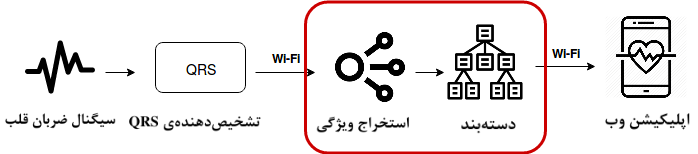
\includegraphics[width=16cm]{Figures/server.png}
\caption{بخش پردازش سمت سرور در مراحل تشخیص آریتمی}
\label{fig:server}
\end{figure}	
	

	\subsection{نحوه‌ی اجرای الگوریتم یادگیری}
		
		\subsubsection{استخراج ویژگی‌ها}
		در فرایند دسته‌بندی ضربان‌‌ها، یک مدل  \lr{SVM} با استفاده از ویژگی‌های استخراج‌شده ساخته می‌شود. همان‌طور که اشاره شد، بازه‌های \lr{RR} و میزان نوسانات آن‌ها ظرفیت بالایی در تشخیص آریتمی دارند، از طرف دیگر، در صورت استفاده از این ویژگی، داده‌های ارسالی از سمت سخت‌افزار متصل به بیمار، حجم پایینی خواهند داشت و در نتیجه تاخیر ارسال داده‌ها به سرور به حداقل خواهد رسید، که برای کاربرد بی‌درنگ ما مناسب‌تر است به همین دلیل از بازه‌های \lr{RR} برای تولید ویژگی‌ها استفاده می‌شود.
برای تولید ویژگی‌ها، با دریافت هر قله‌ی \lr{R} جدید در سرور، مقادیر زیر محاسبه می‌شوند:
\begin{itemize}
	\item \lr{Pre-RR}: این مقدار فاصله‌ی بین ضربان جاری (مربوط به قله‌ی \lr{R} دریافت‌شده و قله‌ی ضربان قبلی را نشان می‌دهد.
	\item \lr{Post-RR}: این مقدار فاصله‌ی زمانی بین قله‌ی R تازه دریافت‌شده و قله‌ی R بعدی را نشان می‌دهد.
	\item \lr{Local-RR}: میانگین ۱۰ مقدار \lr{Pre-RR} گذشته در این مقدار محاسبه می‌شود.
	\item \lr{Global-RR}: میانگین مقادیر \lr{Pre-RR}  تولیدشده در ۱۰دقیقه‌ی گذشته در این مقدار محاسبه می‌شود.
\end{itemize}

	در سرور میانگین هر یک از این چهار مقدار محاسبه شده و با رسیدن مقادیر جدید، به‌روز می‌شود. از این میانگین سپس برای نرمال‌سازی ویژگی‌هایی که تا کنون استخراج شده‌اند استفاده می‌شود، به این صورت که هر یک از این چهار ویژگی به میانگین خود تقسیم شده و چهار ویژگی دیگر را می‌سازند. در انتها ۸ ویژگی از بازه‌های \lr{RR} تولید شده و به مدل دسته‌بند تحویل داده می‌شوند.

		
		\subsubsection{ساخت مدل SVM}
پردازش‌های سمت سرور و الگوریتم \lr{SVM} به کمک زبان پایتون و فریم‌ورک \lr{Django} پیاده‌سازی شدند. زبان پایتون به دلیل پشتیبانی از کتاب‌خانه‌های متنوعی برای پیاده‌سازی انواع الگوریتم‌های یادگیری، برای استفاده در این کاربرد مناسب تشخیص داده شد. برای پیاده‌سازی الگوریتم \lr{SVM} در این زبان، از کتاب‌خانه‌ی scikit-learn استفاده کردیم. برای ساخت و آموزش یک مدل \lr{SVM}، نمونه‌ای از کلاس \lr{SVC} (از کلاس‌های عضو کتاب‌خانه‌ی \lr{scikit-learn} که برای دسته‌بندی‌های چنددسته‌ای استفاده می‌شود) ساخته شده و ویژگی‌های استخراج‌شده از داده‌های آموزش، به علاوه‌ی پارامترهای ضروری برای مدل \lr{SVM} به آن داده شدند. 

	تابع کرنل در این مدل، \lr{RBF} در نظر گرفته شده و پارامترهای مربوط به آن تعیین شده‌است. مقدار گاما در این مدل‌ها برابر با مقدار پیش‌فرض گاما در مدل‌های \lr{SVM} قرار داده شد که مساوی با $\frac{1}{number of features}$ است.
	
برای تعیین پارامتر \lr{C} در این مدل، از روش اعتبارسنجی متقابل ۱۰ لایه‌ای استفاده کردیم. در این روش، پارامتر C از مقدار ۰/۰۰۰۱ تا ۱۰۰۰۰ به صورت لگاریتمی تغییر داده شده و به ازای هر مقدار، معیارهای کارایی محاسبه شدند. اعتبارسنجی متقابل در انتها مقدار ۰/۰۰۱ رابه عنوان بهترین مقدار در این بازه برای پارامتر \lr{C} به دست آورد.
 
سپس مدل ساخته شده و آموزش داده شد. در مرحله‌ی بعد، مدل ساخته شده با کمک توابع کلاس \lr{SVC} بر روی مجموعه‌ داده‌های تست امتحان شدند، و از استراتژی رای‌دهی \lr{OVO}\LTRfootnote{One Versus One} برای این کار استفاده شد که در بخش بعد به تفصیل توضیح داده خواهد شد.
	
		\subsubsection{استراتژی رای‌دهی}
		مدل‌هایی که با استفاده از \lr{SVM} ساخته می‌شوند، تنها برای مسائل دسته‌بندی دودویی\LTRfootnote{Binary classification} قابل استفاده هستند. در این مسائل، هدف جداسازی دو کلاس از داده‌ها است. این محدودیت باعث شده است راه‌حل‌هایی ارائه شود تا بتوان از \lr{SVM} در مسائل دسته‌بندی چندکلاسی نیز استفاده کرد. دو راه‌حل اصلی و پرکاربرد برای حل این گونه مسائل، روش OVO و روش OVR\LTRfootnote{One versus Rest} است. در هر دوی این روش‌ها، مدل \lr{SVM} برای حل مسئله‌ای دودویی آموزش داده می‌شود و سپس با استراتژی‌هایی،‌ این دسته‌بندی به چند کلاس تعمیم داده می‌شود.
		 
در روش \lr{OVR} برای یک مسئله دسته‌بندی \lr{k} کلاسی،‌ به ازای هر کلاس، یک مدل \lr{SVM} آموزش داده می‌شود و تعیین می‌کند آیا یک نمونه به این کلاس تعلق دارد یا به بقیه‌ی کلاس‌ها. در این روش \lr{k} دسته‌بند دودویی داریم که بر روی نمونه‌ها اعمال می‌شوند و در انتهابه ازای هر نمونه، \lr{k} نتیجه به دست می‌آید. 
در روش \lr{OVO} تعداد $\frac{k(k-1)}{2}$ مدل \lr{SVM} دودویی متمایز آموزش داده می‌شود. این تعداد برابر با ترکیب ۲ از \lr{k} کلاس،‌ و به بیان دیگر، تعداد روش‌های انتخاب دو کلاس از بین این \lr{k} کلاس است. هر یک از این مدل‌ها یک جفت از کلاس‌های هدف را دریافت کرده و تشخیص می‌دهد یک نمونه به کدام یک از این دو کلاس تعلق دارد. در این روش به ازای هر نمونه، $C(n, 2)$ نتیجه به دست می‌آید.
در هر دوی این روش‌ها، برای تعیین نتیجه‌ی نهایی دسته‌بندی هر نمونه، یک استراتژی رای‌دهی\LTRfootnote{Voting strategy} مورد نیاز است. روش \lr{OVO} نتایج بهتری در مواردی که داده‌ها نامتعادل هستند از خود نشان داده‌است. همچنین این روش در مواردی که تعداد نمونه‌ها بسیار زیاد است،‌ زمان کمتری برای یادگیری نیاز دارد \cite{Mondejar}. به همین دلیل در این پروژه از \lr{OVO} استفاده شده‌است.

با توجه به این که در این کار‌،‌ ۴ کلاس هدف داریم، در مرحله‌ی یادگیری‌، ۶ مدل دودویی ساخته شده و بر روی هر نمونه اعمال می‌شود. در واقع در این‌جا ۶ ابرصفحه ساخته می‌شود که هرکدام، نمونه‌های  یک جفت از کلاس‌های هدف را از هم تمایز می‌دهد. در انتهای این مرحله،‌ ماتریس تابع تصمیم‌گیری\LTRfootnote{Decision function} تولید می‌شود که طول آن برابر با تعداد نمونه‌های مجموعه‌ی آموزش و عرض آن برابر با ۶ است. بر روی هر یک از این ۶ مقدار تعیین‌شده برای هر نمونه،‌لازم است یک استراتژی رای‌دهی اعمال شود. این استراتژی به صورتی که در ادامه توضیح داده خواهد شد پیاده‌سازی شده‌است.

هر یک از مقادیر تابع تصمیم‌گیری نتیجه‌ی دسته‌بندی بین یک جفت از کلاس‌ها را نشان می‌دهد. این نتیجه را مثبت یا منفی بودن مقدار نشان می‌دهد. با توجه به این مقادیر، کلاسی که بیشترین مقدار مثبت را برای یک نمونه دریافت کرده‌باشد، به عنوان کلاس برگزیده برای آن نمونه انتخاب می‌شود. 

	\subsection{نحوه‌ی پردازش داده‌های دریافت‌شده در سرور}

مراحلی که پیش‌تر توضیح داده شدند، به خصوص اعتبارسنجی متقابل، از نظر محاسبات و زمان اجرا بسیار هزینه‌بر هستند. این بخش‌ها به صورت آفلاین و بر روی کامپیوتر شخصی اجرا شدند. خروجی این مراحل یک مدل \lr{SVM} است که توانایی پیش‌بینی برچسب داده‌‌های ناشناخته و جدید را دارد. کتاب‌خانه‌ی \lr{scikit-learn} این امکان را می‌دهد که مدل \lr{SVM} حساب‌شده، در یک فایل باینری ذخیره شود. هر بار که نیاز به پیش‌بینی برچسب داده‌ی جدیدی بود، مدل \lr{SVM} را می‌توان از روی این فایل بارگیری کرده و با پاس‌دادن ویژگی‌های داده‌های جدید به آن، برچسب‌های پیش‌بینی‌شده را دریافت نمود. هزینه‌ی این کار به طرز چشم‌گیری کم‌تر از این است که مدل هر بار از روی داده‌های آموزش ساخته‌ شده و آموزش داده شود.

 پس از انتخاب بهترین پارامترها به کمک اعتبارسنجی متقابل، ساخت و ارزیابی مدل به صورت آفلاین انجام شد. این مدل بر روی فایل باینری ذخیره شده و به سرور انتقال داده شد. برای پیاده‌سازی عملیات سمت سرور، از محیط توسعه‌ی فراهم‌شده به وسیله‌ی وب‌سایت \url{pythonanywhere.com} استفاده شد. این محیط، قابلیت میزبانی اپلیکیشن‌های وب توسعه‌داده‌شده با پایتون را فراهم می‌کند.
 
 نحوه‌ی عملکرد کد سمت سرور به این صورت است که به محض دریافت داده‌‌های پیش‌پردازش‌شده‌ی جدید از سمت سخت‌افزار، این داده‌ها در پایگاه‌داده‌ی خود سرور ذخیره می‌شوند. سخت افزار برای فرستادن مقدار جدیدی به نام \lr{value} به سرور، هر بار یک درخواست \lr{HTTP} به این شکل زیر به سرور می‌فرستد:
\lr{GET /store/\{value\}}
 
کاربر برای دیدن نتایج پردازش‌ها، کافی است \lr{URL} دامنه را در مرورگر خود وارد کند، و در واقع یک درخواست \lr{HTTP GET} به مسیر / بزند. این درخواست در سرور به این صورت مدیریت می‌شود که ابتدا مدل \lr{SVM} از روی فایل بارگیری شده، سپس آخرین داده‌‌های پیش‌پردازش‌شده که تا کنون در پایگاه‌داده ذخیره شده‌اند، به مدل داده می‌شوند تا کلاس آن‌ها پیش‌بینی شود. سپس نتیجه در مرورگر به کاربر نشان داده خواهد شد. 
 
برای آسان‌تر بودن استفاده برای کاربر، صفحه‌ی وب طراحی شده به صورت خودکار و هر یک ثانیه یک بار بارگیری می‌شود. با فرض این که سخت‌افزار به طور مرتب قله‌های \lr{R} تشخیص‌داده‌شده را برای سرور بفرستد، در هر ثانیه یک درخواست \lr{GET} به مسیر / زده شده و کلاس‌های داده‌های جدید به وسیله‌ی مدل، پیش‌بینی و بر روی صفحه‌ی وب نمایش داده می‌شوند. با توجه به این که به طور تقریبی در هر ثانیه یک ضربان قلب تولید می‌شود، چنین کاربردی به صورت بی‌درنگ و با تاخیری اندک نتایج دسته‌بندی هر ضربان را به کاربر نشان می‌دهد. نمونه‌ای از خروجی نشان‌داده‌شده به کاربر در مرورگر، در شکل \ref{fig:website} قابل مشاهده است.

\begin{figure}[!htb]
\centering
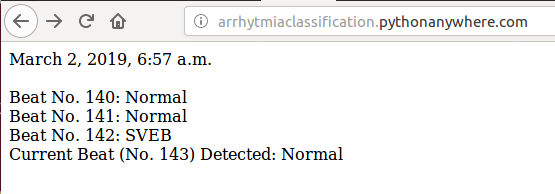
\includegraphics[width=15cm]{Figures/website.png}
\caption{خروجی نشان‌داده‌شده در مرورگر}
\label{fig:website}
\end{figure}	

	\subsection{داده‌های مورد بررسی در الگوریتم یادگیری}
	به منظور استانداردسازی الگوریتم‌های گوناگون تشخیص آریتمی، لازم است ارزیابی این الگوریتم‌ها بر روی مجموعه داده‌های استاندارد و مشترکی صورت بگیرد تا در مقایسه‌ی نتایج حاصل از آن‌ها با دقت کافی حاصل شود. برای این منظور، تعدادی پایگاه‌داده از نمونه‌های ضربان قلب توسط موسسه‌های گوناگون گردآوری شده است. انجمن پیشبرد ابزار دقیق پزشکی\LTRfootnote{Association for the Advancement of Medical Instrumentation (AAMI) } که به اختصار \lr{AAMI} نامیده می‌شود، تعدادی از این پایگاه‌داده‌ها را به عنوان منابع استاندارد داده برای ارزیابی الگوریتم‌های تشخیص آریتمی معرفی کرده و هم‌چنین قراردادهایی برای اجرای عملیات ارزیابی الگوریتم‌ها در آن تعیین کرده‌است، تا کاملا از تکرارپذیری و قابل‌مقایسه‌بودن نتایج آزمایش‌های متفاوت اطمینان حاصل شود. در این استاندارد، استفاده از ۵ پایگاه‌داده‌ی زیر توصیه شده است:
\begin{itemize}
	\item پایگاه‌داده‌ی \lr{MIT-BIH}\LTRfootnote{Massachusetts Institute of Technology - Beth Israel Hospital} شامل ۴۸ نوار قلب ۳۰ دقیقه‌ای
	\item پایگاه‌داده‌ی \lr{EDB}: شامل ۹۰ نوار قلب ۲ ساعته
	\item پایگاه‌داده‌ی \lr{AHA} شامل ۸۰ نوار قلب ۳۵ دقیقه‌ای
	\item پایگاه‌داده‌ی \lr{CU} شامل ۳۵ نوار قلب ۸ دقیقه‌ای
	\item پایگاه‌داده‌ی \lr{NST} شامل ۱۲ نوار قلب ۳۰ دقیقه‌ای
\end{itemize}	 
از بین این موارد، \lr{MIT-BIT} که در این پروژه از آن استفاده کرده‌ایم، اولین پایگاه‌داده‌ی به‌وجودآمده برای این منظور، و پرکاربردترین مجموعه داده برای دسته‌بندی و ارزیابی الگوریتم‌های تشخیص آریتمی است \cite{ECGSurvey}. در ادامه این پایگاه‌داده را دقیق‌تر بررسی خواهیم کرد. 


		\subsubsection{پایگاه‌داده‌ی MIT-BIH}
		برچسب‌گذاری‌های ضربان‌ها در \lr{MIT-BIH} در طی سال‌ها به طور دائم بهبود داده شده‌اند. به دلیل گستردگی داده‌ها و وجود انواع ضربان‌قلب در این نمونه‌‌ها، بیشترین پژوهش‌ها بر روی این پایگاه‌داده‌ انجام گرفته‌اند \cite{ECGSurvey}. 
در \lr{MIT-BIH} تمامی ضربان‌ها به وسیله‌ی یک الگوریتم تشخیص \lr{QRS} از یک‌دیگر متمایز شده‌اند و به هر تک‌ضربان قلب، برچسبی اختصاص داده شده است که نوع آن ضربان  را تعیین می‌کند. این برچسب‌ها در برای پیاده‌سازی و ارزیابی الگوریتم‌های تشخیص آریتمی ضروری هستند. نحوه‌ی انجام این برچسب‌گذاری نیز در استاندارد \lr{AAMI} تعیین شده‌است.

با وجود تنوع انواع ضربان‌قلب‌های دارای آریتمی، ترجیح \lr{AAMI} بر استفاده از ۱۵ کلاس از بین این انواع است. این ۱۵ کلاس، خود به ۵ کلاس کلی‌تر طبقه‌بندی شده‌اند: 
\begin{enumerate}
	\item ضربان‌های عادی\LTRfootnote{Normal} \lr{(N)}
	\item ضربان‌های نابه‌جای فوق بطنی\LTRfootnote{Supraventricular ectopic beats} \lr{(SVEB)}
	\item ضربان‌های نابه‌جای بطنی\LTRfootnote{Ventricular ectopic beats} \lr{(VEB)}
	\item ضربان‌‌های ادغام‌شده\LTRfootnote{Fusion beats} \lr{(F)}
	\item ضربان‌های ناشناخته\LTRfootnote{Unknown beats} \lr{(Q)}
\end{enumerate}

این پایگاه‌داده‌ شامل ۴۸ نوارقلب با نرخ نمونه‌برداری ۳۶۰ هرتز است. این نوارقلب‌ها از ۴۷ بیمار گرفته شده‌اند و هر کدام مدت‌زمانی برابر با ۳۰ دقیقه دارد. هر نوارقلب، شامل نمونه‌های دو لید مجزا است. در بیشتر نوارقلب‌ها، لید اصلی که لید \lr{A} نام دارد، نمونه‌ی تغییریافته‌ای از لید \lr{II} است که از الکترودهای قرارگرفته بر روی سینه به دست می‌آید. لید دوم که لید \lr{B} نام دارد، در بیشتر نوارقلب‌ها لید \lr{V1} و در دیگران \lr{V2}, \lr{V4} و یا \lr{V5} است. عموما برای تشخیص آریتمی از لید اول \lr{(A)} استفاده می‌شود، چرا که در این لید، موج \lr{QRS} واضح‌تر است \cite{ECGSurvey}.

پایگاه‌داده‌های موجود از نظر تعداد ضربان‌های متعلق به هر کلاس آریتمی، شدیدا نامتعادل\LTRfootnote{Imbalanced} هستند. \lr{MIT-BIH} تنها پایگاه‌داده‌ای است که هر ۵ کلاس آریتمی ذکرشده را پوشش می‌دهد. اما در این پایگاه‌داده نیز، حدود ۹۰ درصد ضربان‌ها در کلاس \lr{N} جای می‌گیرند و از ۱۰ درصد باقی‌مانده، حدود ۳٪، ۶٪ و ۱٪ به ترتیب متعلق به کلاس‌های \lr{SVEB}، \lr{VEB} و \lr{F} هستند، و درصد ضربان‌های کلاس \lr{Q} پایین‌تر از ۱ درصد است \cite{Mondejar}. به همین دلیل، لازم است در الگوریتم‌های دسته‌بندی و روش‌های ارزیابی آن‌ها، نامتعادل‌بودن پایگاه‌داده مد نظر قرارگیرد.

		\subsubsection{نحوه‌ی تقسیم داده‌ها به دو مجموعه‌ی آموزش و تست}
		دو الگوی اصلی برای ارزیابی روش‌های اتوماتیک تشخیص آریتمی استفاده می‌شود: الگوی درون‌بیماری\LTRfootnote{Intra-patient paradigm} و الگوی بین‌بیماری\LTRfootnote{Inter-patient paradigm}. در الگوی اول، هیچ‌گونه محدودیتی در تقسیم پایگاه‌داده به دو بخش آموزش و تست وجود ندارد و هر یک از ضربان‌قلب‌های موجود را می‌توان صرف نظر از این که متعلق به کدام بیمار است، در هر یک از این دو مجموعه جای داد. این نوع تقسیم بندی، یک نقص اساسی دراین روش تقسیم‌بندی را موجب می‌شود. از آن جا که در حین یادگیری، امکان دارد مدل تولید شده بتواند الگوهای موجود در ضربان‌های یک بیمار خاص را نیز تشخیص داده و یادبگیرد، نتایج ارزیابی به‌دست‌آمده از الگوریتمی که با الگوی درون‌بیماری کار می‌کند، نمی‌تواند کاملا قابل اعتماد باشد. چرا که به طور مطلوب، یک الگوریتم دسته‌بندی آریتمی باید بتواند برای هر بیماری، با دقتی معین عمل کند، حتی اگر سیستم از پیش اطلاعی در مورد آن بیمار نداشته‌باشد. 
در راستای ارزیابی واقع‌گرایانه‌تر، الگوی بین‌بیماری توسط \lr{Chazal} و همکاران معرفی شد \cite{deChazal2004}. در این الگو تقسیم‌بندی پایگاه‌داده به دو مجموعه‌ی یادگیری و ارزیابی، طوری صورت می‌گیرد که هیچ ضربانی از یک بیمار خاص در هر دو مجموعه به طور هم‌زمان حاضر نباشد. نحوه‌ی تقسیم‌بندی داده‌ها در استاندارد ارائه‌شده به صورت زیر می‌باشد:
\begin{itemize}
	\item مجموعه‌داده‌ی اول \lr{(DS1)} شامل نوارقلب‌های 101, 106, 108, 109, 112, 114, 115, 116, 118,
119, 122, 124, 201, 203, 205, 207, 208, 209, 215, 220, 223 و
230
	\item مجموعه‌داده‌ی دوم \lr{(DS2)} شامل نوارقلب‌های 100, 103, 105, 11, 113, 117, 121, 123,
200, 202, 210, 212, 213, 214, 219, 221, 222, 228, 231, 232, 233
و 234
\end{itemize}
 همان‌طور که اشاره شد، ارزیابی مدل‌ها با استفاده از این الگو، نتایج قابل‌اعتمادتری ارایه می‌کنند. این روش تقسیم‌بندی پس از معرفی، به طور گسترده‌ای در کارهایی که با الگوی بین‌بیماری کار می‌کنند به کار رفته‌است. در این پروژه نیز از این الگو برای ارزیابی بهره گرفته شده‌است. 



	\subsection{ارزیابی نتایج حاصل از یادگیری}
	معیارهای دقت، صحت، صحت کلی و حساسیت (که در بخش \ref{sec:performance} توضیح داده شدند) توسط \lr{AAMI} برای ارزیابی روش‌های مختلف پیشنهاد شده‌اند. 
به دلیل نامتعادل بودن پایگاه‌داده‌های موجود، صحت کلی نمی‌تواند معیار مناسبی برای سنجش باشد. در\lr{MIT-BIH} به دلیل پر تعداد بودن ضربان‌های متعلق به کلاس \lr{N} که حدود ۹۰ درصد داده‌ها را به خود اختصاص داده‌اند،‌ این کلاس در محاسبه‌ی صحت کلی بر دیگر کلاس‌ها شدیدا غالب می‌شود. به همین دلیل، این معیار به طور معمول برای مقایسه‌ی الگوریتم‌ها مورد استفاده قرار نمی‌گیرد.

\subsubsection{معیارهای کارایی}
\label{subsec:perf}
علاوه بر چهار معیار ذکرشده، معیارهای دیگری توسط \lr{AAMI} به عنوان معیارهای استاندارد معرفی شده‌اند. این معیارها از ماتریس درهم‌ریختگی استخراج می‌شوند و طبق  استاندارد‌، استثنائاتی در محاسبه‌ی آن‌ها در نظر گرفته می‌شود. برای مثال، در صورتی که الگوریتم دسته‌بندی، ضربانی از کلاس \lr{F} را به اشتباه متعلق به کلاس \lr{VEB} تشخیص دهد، در میزان موفقیت یا خطای الگوریتم تاثیری نخواهد داشت. 
همان‌طور که ذکر شد، صحت کلی نمی‌تواند میزان موفقیت یک الگوریتم در دسته‌بندی ضربان‌ها را به خوبی نشان دهد. برای غلبه بر این مشکل، یک مقدار جدید به نام اندیس \lr{j$\kappa$} توسط \lr{Mar} و همکاران معرفی شده است \cite{Mar2011}. این مقدار مجموع وزن‌داری از اندیس \lr{j} و کاپای کوهن ($\kappa$) است.

اندیس \lr{j} (رابطه‌ی \ref{eq:jindex}) به پیروی از استاندارد \lr{AAMI}، دقت تمایزدهی مهم‌ترین کلاس‌های آریتمی، یعنی \lr{VEB} و \lr{SVEB} را اندازه‌گیری می‌کند \cite{Mondejar}.
\begin{equation}
	j\:index = Se_{SVEB} + Se_{VEB} + P^+_{SVEB} + P^+_{VEB}
	\label{eq:jindex}
\end{equation}

کاپای کوهن مقداری قراردادی برای ارزیابی نتایج موجود در ماتریس درهم‌ریختگی است. کاپا به عنوان معیاری مقاوم‌تر به نسبت صحت کلی برای پایگاه‌داده‌های نامتعادل گزارش شده‌است. در این رابطه، $P_o$ که احتمال مشاهده‌شده\LTRfootnote{Observed probability} نام دارد، مساوی با صحت کلی است،‌ و مقداری دیگر به نام $P_e$ نیز تعریف می‌شود. در محاسبه‌ی این مقدار، تعداد نمونه‌های موجود در هر کلاس لحاظ شده‌است و به این دلیل برای مقایسه‌ی عملکرد در پایگاه‌داده‌های نامتعادل مناسب است. 

\begin{equation}
\begin{split}
	& \kappa = \frac{P_o - P_e}{1 - P_e} \\
	& P_o = \frac{Nn+Ss+Vv+Ff}{\Sigma} \\
	& P_e = \frac{\Sigma N \Sigma n + \Sigma S \Sigma s + \Sigma V \Sigma v + \Sigma F \Sigma f}{\Sigma^2}
\end{split}
\end{equation}

اندیس \lr{j$\kappa$} به صورت رابطه‌ی \ref{eq:jkindex} محاسبه می‌شود. وجود $\kappa$ باعث می‌شود نرخ دسته‌بندی نادرست\LTRfootnote{Misclassification rate} و همین‌طور تعداد نمونه‌های موجود در هر کلاس در محاسبه‌ی این معیار مد نظر قرارداده شود. به طور هم‌زمان، میزان تشخیص \lr{VEB} و \lr{SVEB} نیز که در محاسبه‌ی اندیس \lr{j} لحاظ شده‌اند،‌ در این مقدار دخالت دارند. تمامی این مقادیر،‌ اندیس \lr{j$\kappa$} را به معیاری مناسب برای مقایسه‌ی الگوریتم‌های دسته‌بندی آریتمی تبدیل کرده است.  
\begin{equation}
	j\kappa\:index = \frac{1}{2}\kappa + \frac{1}{8}(j\:index)
\label{eq:jkindex}
\end{equation}



%------------------------ End chapter 3 -------------


\cchapter{نتایج به‌دست‌آمده }
\label{chap:result}
\pagebreak

در این کار، آزمایش‌هایی با هدف بهینه کردن زمان پاسخ کل الگوریتم و دقت الگوریتم دسته‌بندی انجام شد. هم‌چنین برای ارتباط بهتر کاربران (بیمار و پزشک) با سیستم، یک اپلیکیشن تحت وب برای دسترسی کاربر به نتایج دسته‌بندی طراحی و پیاده‌سازی شد. در ادامه به نتایج به‌دست‌آمده در این بخش‌ها می‌پردازیم.

\section{زمان پاسخ سیستم}
در این کاربرد، زمان پاسخ را مدت‌زمان بین تولید یک ضربان قلب در سیگنال نوار قلب، تا لحظه‌ای که کلاس آن ضربان به کاربر نشان داده می‌شود در نظر گرفته‌ایم. این زمان معیاری برای بررسی سرعت و میزان کارآمدبودن سیستم، به عنوان یک سیستم بی‌درنگ بوده و از این جهت اهمیت بالایی دارد. 

همان‌طور که پیش‌تر توضیح داده شد،در ابتدا سخت‌افزار با دریافت یک ضربان قلب، الگوریتم تشخیص \lr{QRS} را بر روی آن اجرا کرده و قله‌ی \lr{R} را در ضربان تشخیص می‌دهد. مدت‌زمانی که طول می‌کشد تا این عمل انجام شود را $t_{QRS}$ نامیده‌ایم. این زمان به طور متوسط ۳۲۰ میکروثانیه محاسبه شد که به دلیل ناچیزبودن در برابر زمان‌های محاسبه‌شده‌ی دیگر، در محاسبات لحاظ نشد. سخت‌افزار پس از تشخیص یک قله‌ی ‌\lr{R} آن را بلافاصله برای سرور می‌فرستد. این مدت‌زمان، زمان ارسال به سرور ($t_{send}$) نامیده شده و به طور متوسط برابر با ۰/۶ ثانیه محاسبه شده است.

قله‌ی \lr{R} تشخیص‌داده‌شده به محض رسیدن به سرور، در پایگاه‌داده ذخیره خواهد شد. مدل زمان انجام این عمل که $t_{store}$ نام دارد در  بدترین حالت ۳۰ میلی‌ثانیه به دست آمد. برای دیدن نتیجه‌ی هر ضربان، لازم است صفحه دوباره بارگذاری شده و عملیات پیش‌بینی انجام شود. صفحه با نرخ یک بار در ثانیه بارگذاری می‌شود و در بدترین حالت، یک ثانیه بعد درخواستی برای پیش‌بینی برچسب ضربانی که هم اکنون در سرور ذخیره شده‌است، از طرف مرورگر به سرور داده خواهد شد. این زمان را $t_{refresh}$ می‌نامیم.

پس از ارسال درخواست، سرور مدتی را صرف پردازش داده‌ی جدید و نمایش نتیجه در صفحه‌ی وب می‌کند. این مدت زمان که $t_{predict}$ نامیده شد نیز در بیشترین حالت ۵۰ میلی‌ثانیه به دست آمد. به این ترتیب می‌توان کل مدت‌زمان پاسخ را طبق معادله‌ی \ref{eq:responseTime} محاسبه کرد.

\begin{equation}
\begin{split}
	& t_{response} = t_{send} + t_{store} + t_{refresh} + t_{predict} \\
	& = 600 ms + 30 ms + 1 s + 50 ms = 1/680 s
\end{split}
\label{eq:responseTime}
\end{equation}
به این ترتیب مدت‌زمانی کم‌تر از ۲ ثانیه برای زمان پاسخ ضمانت می‌شود.
 
\section{معیارهای کارایی نهایی الگوریتم دسته‌بندی}
همان طور که در بخش \ref{subsec:perf} اشاره شد، مهم‌ترین معیاری که در این کار برای سنجش میزان موفقیت الگوریتم دسته‌بندی مورد استفاده قرار دادیم، اندیس \lr{j$\kappa$ } است. روش اعتبارسنجی متقابل مقدار  ۰/۰۰۱ را به عنوان بهترین مقدار برای پارامتر \lr{C} تعیین نمود. پس از قراردادن این مقدار برای \lr{C} و ساخت و ارزیابی مدل، مقدار اندیس \lr{j$\kappa$ } برابر با ۰/۴۲۸ به دست آمد. در جدول ۱-۴ مقادیر به‌دست‌آمده برای دیگر معیارهای کارایی مشاهده می‌شوند. 

 ماتریس درهم‌ریختگی حاصل به صورت جدول ۲-۴ است. با نگاه به این ماتریس در می‌یابیم تعداد زیادی از ضربان‌های عادی به صورت ضربان‌های 
\lr{F} تشخیص داده شده‌اند. این امر به معنای دقت پایین در تشخیص کلاس \lr{F} است که مهم‌ترین ضعف مشاهده‌شده در نتایج به دست آمده می‌باشد.



علاوه بر این نتایج، مقدار $\kappa$ برابر با ۰/۳۵۶۷ و مقدار اندیس \lr{j } برابر با ۱/۹۹۹۸ به دست آمد. همان طور که اشاره شد، اندیس  \lr{j$\kappa$} به کمک معادله‌ی \ref{eq:jkindex} با استفاده از این مقادیر محاسبه می‌شود.


\begin{table}
\begin{center}
\begin{latin} 
\begin{tabular}{l*{6}{c}r}
Beat Class              & Sensitivity & Precision & Accuracy  \\
\hline
N & 0.7657 & 0.9865 & 0.7831  \\
SVEB            & 0.4717 & 0.2653 & 0.9243  \\
VEB           & 0.7854 & 0.4773 & 0.9299  \\
F    & 0.9201 & 0.0572 & 0.8809  \\
Mean    & 0.7357 & 0.4466 & 0.8796  \\
\end{tabular}
\end{latin}
\caption{نتایج دسته‌بندی در کلاس‌های مختلف ضربان و به صورت میانگین}
\end{center}
\label{table:results}
\end{table}

\begin{table}
\begin{center}
\begin{latin}
  \begin{tabular}{  l | c | r | r | r |}
    
     & N & SVEB & VEB & F \\ \hline
    N & 33718 & 2398 & 2386  & 5531\\ \hline
    SVEB & 349 & 967 & 707 & 27 \\ \hline
    VEB & 85 & 279 & 2529 & 327 \\ \hline
    F & 27 & 1 & 3 & 357 \\  \hline
  \end{tabular}
  
\end{latin}
\caption{ماتریس درهم‌ریختگی نتیجه}
\end{center}
\label{table:confmat}
\end{table}

برای به‌دست‌آوردن دید بهتری از میزان موفقیت این روش، به بالاترین مقدار اندیس \lr{j$\kappa$ } به‌دست‌آمده در کارهای گذشته اشاره می‌کنیم که برابر با ۰/۶۶۳ می‌باشد \cite{Mar2011}. دلیل پایین‌تر بودن اندیس \lr{j$\kappa$ } به ‌دست‌ آمده در این پروژه نسبت به این مقدار، استفاده از ویژگی \lr{RR} به تنهایی می‌باشد. در کارهایی که بالاترین مقادیر اندیس \lr{j$\kappa$ } را به‌دست‌آورده‌اند، از ویژگی‌های دیگری نیز علاوه بر بازه‌های \lr{RR} استفاده شده‌است. برای مثال در  \cite{Zhang2014} از ویژگی‌های بازه‌های \lr{RR} و هم‌چنین ویژگی‌های مربوط به شکل موج‌های ضربان قلب استفاده شده‌است. در \cite{deChazal2004} از ویژگی‌های شکل موج ضربان و ویژگی‌های استخراج شده از فواصل ضربان‌ها نیز علاوه بر بازه‌های \lr{RR} به کار گرفته شده و اندیس \lr{j$\kappa$ } برابر با ۰/۶۱۲ به دست آمده‌است.
 
در \cite{Mondejar} از بازه‌ی RR به تنهایی به عنوان ویژگی استفاده شده و مقدار ۰/۴۳۹ برای اندیس \lr{j$\kappa$ } به‌ دست‌ آمده‌است، که به مقداری که ما به دست آورده‌ایم نزدیک می‌باشد. 





 
\cchapter{نتیجه‌گیری و کارهای آینده}
\label{chap:conclusion}
\pagebreak
در این کار، یک سیستم تشخیص و دسته‌بندی آریتمی قلبی پیاده‌سازی شد. این سیستم توانایی کارکردن به صورت بی‌درنگ را دارد و در طول مدت‌زمان کم‌تر از ۲ ثانیه، کلاس آریتمی ضربان دریافت‌شده را تشخیص می‌دهد. دقت الگوریتم دسته‌بندی پیاده‌سازی‌شده به طور میانگین ۰/۴۴ به دست آمد، هم‌چنین حساسیت میانگین این دسته‌بندی ۰/۷۳ و  \lr{j$\kappa$ index} آن ۰/۴۳ محاسبه شد. 

این سیستم به دو بخش کلی پیش‌پردازش بر روی سخت‌افزار و پردازش اصلی بر روی سرور تقسیم می‌شود. بخش اول بر روی یک ماژول \lr{ESP8266} پیاده شد که باید به یک سنسور دیجیتال ضربان قلب متصل شود. در این بخش یک الگوریتم تشخیص \lr{QRS} با روش پن-تامپکینز و با هدف تشخیص قله‌های \lr{R} هر ضربان بر روی سیگنال نوار قلب اجرا شد و نتیجه‌ی این پیش‌پردازش به سرور ارسال گردید.

در بخش دوم، یک مدل دسته‌بندی \lr{SVM} به صورت آفلاین آموزش داده شد و سپس مدل آموزش‌داده‌شده به صورت فایل ذخیره شده و به سرور انتقال داده شد. یک کد سمت سرور برای دریافت درخواست‌ها و پیش‌بینی کلاس ضربان‌‌های جدید پیاده‌سازی شد.

الگوریتم دسته‌بندی بر روی پایگاه‌داده‌ی \lr{MIT-BIH} اجرا شد و برای تقسیم داده‌های این پایگاه‌داده به دو مجموعه‌ی آموزش و تست، از الگوی بین‌بیماری بهره گرفته شد. برای ارزیابی کارایی این دسته‌بندی، از معیار اندیس  \lr{j$\kappa$} استفاده شد که نمای مناسبی از میزان کارایی یک الگوریتم دسته‌بندی آریتمی ارایه می‌کند.

از مهم‌ترین نیازمندی‌های این پروژه، سرعت بالا و بی‌درنگ بودن تشخیص آریتمی است که با توجه به زمان پاسخ به‌دست‌آمده، می‌توان گفت این نیازمندی برآورده شده‌است. هم‌چنین قابل‌حمل‌بودن سخت‌افزار همراه بیمار  از نیازمندی‌های دیگر بود که با پیاده‌سازی بخش سخت‌افزاری کار بر روی ماژول \lr{ESP8266} که حجم و مساحت کوچکی دارد، تا حد خوبی برآورده شده‌است.

نیازمندی دیگر این کار، دقت بالای الگوریتم دسته‌بندی ذکر شد. در این کار در مرحله‌ی استخراج ویژگی، تنها از بازه‌های \lr{RR} ضربان‌های قلب استفاده شد و ویژگی‌هایی با استفاده از این بازه‌ها استخراج شدند. دلیل این امر، کارایی بالایی بود که این ویژگی‌ در کارهای گذشته از خود نشان داده‌است. حجم پایین ویژگی‌های استخراج شده و سبک‌تر بودن محاسبات مورد نیاز بر روی سخت‌افزار همراه بیمار  نیز باعث شد ویژگی \lr{RR} مناسب تشخیص داده شود، چرا که ما را به هدف بی‌درنگ‌بودن سیستم و قابل‌حمل‌بودن سخت‌افزار آن نزدیک می‌نماید.

اندیس  \lr{j$\kappa$} به دست آمده در این پروژه، ۰/۴۲۸ است که به نسبت بالاترین اندیس  \lr{j$\kappa$} های به دست آمده در کارهای گذشته (۰/۶۶۳ در \cite{Mar2011}) مقداری پایین‌تر است، اما به نسبت بالاترین مقداری که تنها با استفاده از ویژگی \lr{RR} حاصل شده‌است (۰/۴۳۹ در \cite{Mondejar}) مقداری مناسب است. پس می‌توان گفت به طور کلی به نیازمندی دقت و حساسیت بالای سیستم پاسخ کامل داده نشده‌است، و دلیل این امر، استفاده از ویژگی \lr{RR} به تنهایی بوده‌است.


در کارهای آینده می‌توان از چند مدل \lr{SVM} که هر یک با یک مجموعه از ویژگی‌ها آموزش داده شده اند و ترکیب نتایج آن‌ها، برای ساخت یک مدل \lr{SVM} قوی‌تر بهره برد. در کار پیش رو، در مرحله‌ی تشخیص \lr{QRS}، تنها از ولتاژ یک لید (\lr{MLII}) استفاده شد که واضح‌ترین ترکیب \lr{QRS} را بین لیدهای قلبی نمایش می‌دهد. در آینده می‌توان الگوریتم‌هایی طراحی نمود که از  لیدهای بیشتری بهره می‌برند، و تاثیر این کار را بر بالارفتن دقت تشخیص \lr{QRS} بررسی کرد.


\newpage

%\begin{latin}
\pagestyle{plain}
{
\onehalfspacing
\bibliographystyle{ieeetr-fa}%{chicago-fa}%{plainnat-fa}%
\bibliography{Thesis}
}
%\end{latin}

\newpage

%include{appendix}

\begin{latin}
%\latinfirstPage
\end{latin}
\end{document} 
